% SPDX-FileCopyrightText: 2023 SAP SE
%
% SPDX-License-Identifier: Apache-2.0
%
% This file is part of FEDEM - https://openfedem.org

%%%%%%%%%%%%%%%%%%%%%%%%%%%%%%%%%%%%%%%%%%%%%%%%%%%%%%%%%%%%%%%%%%%%%%%%%%%%%%%%
%
% FEDEM User Guide.
%
%%%%%%%%%%%%%%%%%%%%%%%%%%%%%%%%%%%%%%%%%%%%%%%%%%%%%%%%%%%%%%%%%%%%%%%%%%%%%%%%

\def\RightFigure#1#2{\noindent
  \begin{minipage}{0.65\textwidth}
    \raggedright#2
  \end{minipage}% <--- the % is needed here to kill off spurious spacing
  \hfill\begin{minipage}{0.25\textwidth}
    \includegraphics[width=0.8\textwidth]{Figures/#1}
  \end{minipage}}

% Temporary, to aid setting picture encironment sizes
\def\Hline#1{\put(0,0){\line(1,0){#1}}}
\def\Vline#1{\put(0,0){\line(0,1){#1}}}


\Chapter{Mechanism Elements}{mechanism-elements}

Now that you know how to create and assemble
mechanism elements, you need to
know how Fedem defines the properties of elements and how you can
customize them to suit your design requirements. This chapter presents
each of the mechanical and modeling elements used in Fedem mechanisms.
It also describes each element's properties and how they can be edited
once the element is created.

Sections in this chapter address the following topics:

\begin{itemize}
\item
  \protect\hyperlink{parts}{Parts}
\item
  \protect\hyperlink{element-groups}{Element groups}
\item
  \protect\hyperlink{beams}{Beams}
\item
  \protect\hyperlink{beam-cross-sections}{Beam cross sections}
\item
  \protect\hyperlink{triads}{Triads}
\item
  \protect\hyperlink{joints}{Joints}
\item
  \protect\hyperlink{joint-pair-constraints}{Joint pair constraints}
\item
  \protect\hyperlink{frictions}{Frictions}
\item
  \protect\hyperlink{springs-and-dampers}{Springs and Dampers}
\item
  \protect\hyperlink{loads}{Loads}
\item
  \protect\hyperlink{functions}{Functions}
\item
  \protect\hyperlink{sensors}{Sensors}
\item
  \protect\hyperlink{strain-rosettes}{Strain rosettes}
\item
  \protect\hyperlink{generic-database-objects}{Generic database objects}
\item
  \protect\hyperlink{sub-assemblies}{Sub-assemblies}
\end{itemize}

\clearpage

%%%%%%%%%%%%%%%%%%%%%%%%%%%%%%%%%%%%%%%%%%%%%%%%%%%%%%%%%%%%%%%%%%%%%%%%%%%%%%%%
\input{Parts}


%%%%%%%%%%%%%%%%%%%%%%%%%%%%%%%%%%%%%%%%%%%%%%%%%%%%%%%%%%%%%%%%%%%%%%%%%%%%%%%%
\Section{Element groups}{element-groups}

When a part is created by importing a FE model into Fedem,
several element groups might be created as well, see
\refSection{creating-parts-by-file-import}{Creating parts by file import}.
The element groups can be of the following two types:

\begin{itemize}
\item
  \textbf{Explicit groups} : User-defined group through Nastran SETs on
  bulk data files or Fedem GROUPs on \File{.ftl} files.
\item
  \textbf{Implicit groups} : An implicit element group consists of all
  elements referring to one particular material (PMAT) or thickness
  (PTHICK) property record in the FE model file. The ID numbers of these
  groups correspond to the ID numbers of the associated property record.
  Implicit groups are created only for property records that are in use.
\end{itemize}

\Note{When the imported FE model file is a Nastran bulk data file, the created
  PMAT and PTHICK groups correspond to the MAT1 and PSHELL bulk entries,
  respectively, with corresponding ID numbers.
  No implicit groups are created for PSOLID bulk entries.}

\begin{wrapfigure}[12]{r}{0.35\textwidth}
  \includegraphics[trim=0 75 0 0,clip,scale=0.5]{Figures/4-ElementGroups}
\end{wrapfigure}

The element groups are visible in {\sl Objects} list of the Model Manager panel
under each Part node, as shown to the right.
They can be used to control component appearance (see
\refSection{visualizing-the-model}{Visualizing the model}),
and calculation focus (see
\refSection{part-and-group-wise-solving}{Part- and group-wise solving}).

The element groups are also used to assign properties needed in Fatigue
analyses during Strain Coat Recovery simulations (see
\refSection{element-group-properties}{Element group properties} below, and
\refSection{strain-coat-analysis-1}{Strain coat analysis}).

Some Nastran bulk data files may also contain a user-defined name of an
element set or physical property as a comment line before the
set/property definition itself. When found, such comments are parsed and
used in the default description of the created element group when
the bulk data file is imported into Fedem.

\Note{The syntax of the comment lines containing names on element sets and
  properties depends on the software package that produced the actual
  Nastran bulk data file. Currently the syntax of the following packages
  are supported: I-DEAS, Hypermesh and NX.}

\Tip{The description field can be edited both for explicit and implicit
  element groups. The modified description is then stored in the part file
  (\File{.ftl} file). To revert to the original description (e.g. PTHICK for
  implicit groups based on the thickness element property), delete the
  description text completely. Any user-defined name parsed from a Nastran
  bulk data comment line is not restored, however.}


\SubSection{Element group properties}{element-group-properties}

When an element group is selected in the Model Manager panel,
its properties are displayed in the Property Editor panel (shown below).
It contains parameters and settings that are used in Fatigue calculations
during a Strain Coat analysis on this element group.
See \refSection{strain-coat-analysis-1}{Strain coat analysis}
to learn more about such fatigue analyses.

\begin{figure}[H]
  \begin{picture}(343,40)
    \put(0,0){\includegraphics[width=\textwidth]{Figures/4-ElementGroupProperties}}
    \put(-10,14){\Bullet{1}}
    \put(80,4){\Bullet{2}}
    \put(160,4){\Bullet{3}}
    \put(320,4){\Bullet{4}}
  \end{picture}
\end{figure}

\begin{bulletlist}
\item This toggle enables rainflow analysis and fatigue calculations
  for the selected element group.
\item{\sl Standard} --
  Select the fatigue standard to use for in the fatigue calculations.
\item{\sl S-N curve} --
  Select an S-N curve from the selected fatigue standard.
\item{\sl Stress concentration factor} --
  The computed stresses are scaled by this value before they are used in
  the fatigue calculation.
\end{bulletlist}

\Tip{The S-N curve standards available in the pull-down menu are defined in the
  file \File{sn\_curves.fsn} located in the installation directory of Fedem.
  The syntax of the S-N curve definitions is description in the header of this
  file, and it is possible to add your own S-N curve definitions to that file.}

For details on how damage is calculated from a given time history response,
see the \FedemVer~Theory Guide.

\clearpage


%%%%%%%%%%%%%%%%%%%%%%%%%%%%%%%%%%%%%%%%%%%%%%%%%%%%%%%%%%%%%%%%%%%%%%%%%%%%%%%%
\Section{Beams}{beams}

A beam is a flexible body, represented by a standard two-noded beam
finite element. Its stiffness matrix is based on Euler-Bernoulli beam
theory, quadratic interpolation functions and continuous rotations at
the nodal points. The deformations in such elements account for bending,
shear, axial compression and elongation, and St. Venants torsion. The
cross section properties are assumed constant along the beam element.

Beam elements may be used in a Fedem mechanism model, in much the same
way as a generic part connected to two triads. A triad needs to be
placed at each end of a beam element. However, an arbitrary number of
beam elements may be connected at one triad, such that it is possible to
represent a curved (or straight) beam string and 3D space frames.


\SubSection{Creating beams}{creating-beams}

To manually create one or a set of beam elements, proceed as follows:

\vskip20mm
\IconText{beam}{\vspace*{-19mm}
  \begin{enumerate}
    \setlength\itemsep{1mm}
  \item
    Create Triads where you want to locate the nodes of the beam(s).
  \item
    Select two or more triads that should represent the nodes of the beams
    using the multi-select features of Fedem (see \refSection{model-manager}
    {Model Manager} and \refSection{select}{Select}).
  \item
    Click the \textbf{Create Beam} button on the \textbf{Mechanism Creation}
    tool bar, or select it from the \textbf{Mechanism} menu.
  \end{enumerate}}

A set of ({\sl nT}-1) beam elements is then created, where {\sl nT}
denotes the number of selected triads. When three or more triads are
selected, the second triad will become the second node of the first
element created and also the first node of the second element. The third
triad will next become the second node of the second element and the
first node of the third element, and so on. This can therefore be
utilized to create strings of beam elements of any shape and length.

\Note{The newly created beam elements have no cross section properties assigned.
  This needs to be done from the Property Editor panel when one or a group of
  beams is selected (see \refSection{beam-properties}{Beam properties}),
  before the simulation is started.}

\clearpage
\SubSection{Splitting beams}{splitting-beams}

An existing beam element may be divided into an arbitrary number of
beams of uniform length, by using the \textbf{Split Beam...} command:

\vskip11mm
\IconText{splitBeam}{\vspace*{-10mm}
  \begin{enumerate}
    \setlength\itemsep{3mm}
  \item
    Select the beam you want to split from the {\sl Modeler} view
    (or the {\sl Objects} list of the Model Manager panel).
  \item
    On the \textbf{Edit} menu (or the right-click menu),
    select \textbf{Split Beam...}
\end{enumerate}}
\begin{minipage}{0.62\textwidth}
  \raggedright
  \begin{itemize}
  \item[3.]
    A small dialog box then pops up (shown to the right), in which you may enter
    the number of elements that you want the selected element divided into.
  \end{itemize}
\end{minipage}% <--- the % is needed here to kill off spurious spacing
\hfill\begin{minipage}{0.35\textwidth}
  \includegraphics[width=\textwidth]{Figures/Dialogs/4-SplitBeam}
\end{minipage}

If you, e.g., type the value 10 and press \textbf{OK} (or hit the
\textbf{Enter} key), then 9 new beam elements are created, inheriting
all properties of the selected beam, which then will become the first of
the 10 smaller elements that replace the selected element. This can be
used to refine the discretization of a beam string when that is needed
to obtain proper solution accuracy, for instance, due to complicated
load patterns from hydrodynamic loads.

The \textbf{Split Beam...} command may also be applied repeatedly on the same
beam string to obtain graded refinements in a localized area of the beam.


\SubSection{Beam properties}{beam-properties}

When a beam is selected in the Model Manager panel, its properties are
displayed in the Property Editor panel (shown below).

\begin{figure}[H]
  \begin{picture}(343,75)
    \put(0,0){\includegraphics[width=\textwidth]{\ReferenceImg/prp/beam-1}}
    \put(50,57){\Bullet{1}}
    \put(70,30){\Bullet{2}}
    \put(43,14){\Bullet{3}}
    \put(165,68){\Bullet{4}}
    \put(305,68){\Bullet{5}}
    \put(175,33){\Bullet{6}}
  \end{picture}
\end{figure}

\begin{bulletlist}
\item{\sl Cross-section:} --
  This pull-down menu enables the selection of the cross section object
  to be associated with this beam element, see
  \refSection{beam-cross-sections}{Beam cross sections} below.

\item{\sl Mass and Length} --
  Displays the length and the total mass of the beam element.
  The length is computed from the coordinates of the end triads of the beam.
  The mass is computed from the beam length, and the cross section area and mass
  density that is assigned to the beam via the cross section object.
  These fields are updated automatically if any of the referred property objects
  are changed.

\item{\sl Visualize 3D} --
  This toggle enables a 3D visualization of the beam, using the cross section
  parameters to render its actual geometry.
  The default visualization is a straight line connecting the two triads,
  with coloring depending on the referred cross section object.
  The {\sl Start} and {\sl Stop} fields are used to specify a sector of partial
  3D visualization. They define the start and stop angles (in degrees),
  relative to the local $Y$-axis of the cross section,
  of the sector that is to be rendered in 3D.

\item{\sl Structural damping} --
  Allows you to change the values of both the mass and stiffness proportional
  damping for the beam. These fields are equivalent to similar fields in the
  \protect\hyperlink{part-tab}{\sl Part tab} of the Part Property Editor panel,
  see \refSection{part-properties}{Part properties}.

\item{\sl Scaling of dynamic properties} --
  Allows you to scale stiffness and mass of each individual part in the
  dynamics simulation. These fields are equivalent to similar fields in the
  \protect\hyperlink{part-tab}{Part tab} of the Part Property Editor panel,
  see \refSection{part-properties}{Part properties}.

\item{\sl Local Z-axis definition} --
  These three fields allow you to define a vector defining the local $Z$-axis
  of the local coordinate system of the beam. This vector is defined in the
  coordinate system of the parent sub-assembly of the beam,
  or in the global coordinate system in case of no parent assembly.
  The local $Y$-axis is then defined as the cross product between the $Z$-axis
  and the local $X$-axis, the latter being the unit vector from end 1 towards
  end 2 of the beam element.

\EnumNote{If the specified vector is parallel to the local $X$-axis, or if only
  $0.0,0.0,0.0$ is specified, a globalized coordinate system is used instead
  in which the local $Z$-axis is chosen to be as close as possible to the
  global $Z$-axis.}
\end{bulletlist}

\clearpage


%%%%%%%%%%%%%%%%%%%%%%%%%%%%%%%%%%%%%%%%%%%%%%%%%%%%%%%%%%%%%%%%%%%%%%%%%%%%%%%%
\Section{Beam cross sections}{beam-cross-sections}

Beam cross sections are used to describe the cross section properties of a
beam element, see \refSection{beam-properties}{Beam properties}. When a Beam
cross section is selected in the Object browser, its properties are
displayed in the Property Editor panel, as shown below.

\begin{figure}[H]
  \begin{picture}(343,205)
    \put(0,105){\includegraphics[width=\textwidth]{\ReferenceImg/prp/beam-cross-section-1}}
    \put(0,0){\includegraphics[width=\textwidth]{\ReferenceImg/prp/beam-cross-section-2}}
    \put(30,170){\Bullet{1}}
    \put(120,170){\Bullet{2}}
    \put(60,140){\Bullet{3}}
    \put(330,181){\Bullet{5}}
    \put(230,120){\Bullet{8}}
    \put(40,65){\Bullet{1}}
    \put(130,25){\Bullet{4}}
    \put(230,56){\Bullet{7}}
    \put(230,12){\Bullet{8}}
  \end{picture}
\end{figure}

\begin{bulletlist}
\item{\sl Cross section type} --
  This pull-down menu enables the selection of the cross section type.
  Currently you can select {\sl Pipe} or {\sl Generic}.

\item{\sl Material} --
  This pull-down menu enables the selection of the material property object that
  this cross section is to be associated with,
  see \refSection{material}{Material} below. The material selection is
  not available for the {\sl Generic} cross section type, as the material
  properties then are embedded in the other cross section parameters.

\item{\sl Definition} --
  Depending on the cross section type, you will have various fields for defining
  the cross section geometry. For {\sl Pipe} sections, you specify the outer
  ({\sl Do}) and inner ({\sl Di}) diameters only.

\item For {\sl Generic} cross sections,
  you specify the axial stiffness ({\sl EA}),
  the bending stiffnesses ({\sl EIyy} and {\sl EIzz}),
  the torsional stiffness ({\sl GIt}),
  the mass per unit length ($\rho${\sl A})
  and the torsional moment of inertia ($\rho${\sl Ip}).

\item{\sl Dependent properties} --
  These properties (the cross section area, {\sl A},
  and the moments of inertias, {\sl Ip}, {\sl Iyy} and {\sl Izz})
  are updated automatically based on the specified geometry parameters.
  However, if the {\sl Break dependence} toggle is enabled,
  any of the dependent properties may be overridden manually.

\item{\sl Shear reduction factors} --
  These values specify the ratio between the effective transverse shear area and
  the actual cross section area, in the local $Y$- and $Z$-axis directions,
  respectively. Refer to text books on structural mechanics on how these
  parameters depend on different cross section shapes.
  If these values are set to zero, the transverse shear deformation is ignored
  in the FE model(infinite shear stiffness).

\item{\sl Shear stiffness} --
  For {\sl Generic} cross section, you specify the shear stiffness ({\sl GAs,y}
  and {\sl GAs,z}) directly, instead of the shear reduction factors.
  Non-positive values in these fields will be interpreted as infinite
  shear stiffness (no shear deformation).

\item{\sl Shear center offset} --
  These fields allow you to specify the local position of the shear centre of
  the cross section with respect to its elastic centre (or the neutral axis).
  The shear centre defines the point through which a transverse load must be
  act in order to avoid torsional deformation in the beam element.
  For symmetric cross sections the shear centre coincides with the elastic
  centre and the values 0.0 are appropriate.
\end{bulletlist}


\SubSection{Material}{material}

Materials are used to describe material properties of beam elements (linear
isotropic material law only). They are referred to via the Beam cross section
objects described above. When a Material is selected in the Object browser,
its properties are displayed in the Property Editor panel, as shown below.

\medskip\noindent
\begin{minipage}{0.45\textwidth}
  \includegraphics[width=\textwidth]{\ReferenceImg/prp/material-1}
\end{minipage}%
\begin{minipage}{0.5\textwidth}
  \begin{itemize}
  \setlength\itemsep{1mm}
  \item$\rho$ -- Mass density
  \item$E$    -- Young's modulus of elasticity
  \item$\mu$  -- Poisson's ratio
  \item$G$    -- Shear modulus of elasticity
  \end{itemize}
\end{minipage}

\Note{Only one of the parameters $\mu$ and $G$ needs to be specified,
  as they are connected through the relation $G=E/(2+2\nu)$. Whenever you
  change one of these values, the other value will update automatically.}


\clearpage
\SubSection{Import of generic cross sections}{import-of-generic-cross-sections}

The Fedem installation is equipped with a database of predefined beam
cross sections and materials, which can be used to quickly load the
cross section properties of your need into the model.

\vskip\parskip
\IconText{beamCrossSection}{
  To access this database, select \textbf{Import Beam Cross Sections...} from
  the \textbf{File} menu.
  The Cross Section Import dialog box (shown below) pops up.}

\begin{figure}[!h]
  \center
  \includegraphics[width=0.55\textwidth]{Figures/Dialogs/4-ImportCrossSection}
\end{figure}

You can here select one (or more, hold down the \textbf{Shift} or \textbf{Ctrl}
key to multi-select) items from the {\sl Beam cross sections} list,
together with one item from the {\sl Materials} list, and press the
\textbf{Import} button to generate generic beam cross section objects
in your model with those properties.

The cross section database is stored as a set of \File{.csv} files
(tab-separated columns) in the \File{Properties/CrossSections} sub-folder
in your Fedem installation. Each line in these files correspond to one
item in the Cross Section Import dialog box, and there is typically one
file for each group of cross section types. You may easily expand the
cross section database by creating files with similar format placed in a
\File{CrossSections} sub-folder in the home directory of your user profile.
They will then be appended to the pre-installed list of cross sections
when you open this dialog box.


%%%%%%%%%%%%%%%%%%%%%%%%%%%%%%%%%%%%%%%%%%%%%%%%%%%%%%%%%%%%%%%%%%%%%%%%%%%%%%%%
\input{Triads}
% SPDX-FileCopyrightText: 2023 SAP SE
%
% SPDX-License-Identifier: Apache-2.0
%
% This file is part of FEDEM - https://openfedem.org

%%%%%%%%%%%%%%%%%%%%%%%%%%%%%%%%%%%%%%%%%%%%%%%%%%%%%%%%%%%%%%%%%%%%%%%%%%%%%%%%
%
% FEDEM User Guide.
%
%%%%%%%%%%%%%%%%%%%%%%%%%%%%%%%%%%%%%%%%%%%%%%%%%%%%%%%%%%%%%%%%%%%%%%%%%%%%%%%%

\Section{Joints}{joints}

As with real mechanisms, you may connect one part or beam to another using
{\sl joints}. A joint introduces motion and/or spring constraints between the
two parts it is acting between. These constraints are applied on the
{\sl joint DOFs}, also called {\sl Joint Variables}.
Each Fedem joint uses at least two triads to connect the joint to parts.
One or more of the joint's triads are labeled {\sl master} while one triad
is labeled {\sl slave}, with the constrained DOFs of the slave triad following
the movement of the master(s).
(See the \FedemTGuide{Chapter 6, "Modeling of Joints"}.)

To attach a joint to parts, the joint's master triad is attached
to an FE node on one part and the slave triad to an FE node on another part.
This means that when the mechanism moves, the FE node (and part) on the slave
side of the joint follows the motion of those on the master side.
FE nodes and parts can, therefore, also be referred to as masters and slaves.
See \refSection{attaching-and-detaching-elements}
{Attaching and detaching elements} and
\refSection{using-the-attach-command}{Using the Attach command}
about how to attach joints.

\Tip{To determine which triad is the master and which is the slave,
  select one of the parts or the joint to examine the {\sl Topology} view
  of master and slave triads connected to the part/joint.
  You can then select (click and hold down the mouse button) the master/slave
  triad to highlight it in the Modeler view.}


%%%%%%%%%%%%%%%%%%%%%%%%%%%%%%%%%%%%%%%%%%%%%%%%%%%%%%%%%%%%%%%%%%%%%%%%%%%%%%%%
\SubSection{Joint variables}{joint-variables}

The joint variables are the accessible or controllable DOFs for each joint.
As an example, the Revolute Joint normally has one accessible DOF,
namely the rotation about one axis. The other DOFs are fixed.
For most joints the DOFs that are not accessible are fixed,
but for Prismatic and Cylindrical joints that is not the case.
Refer to \protect\hyperlink{prismatic-joint}{\sl"Prismatic joint"} and
\protect\hyperlink{cylindric-joint}{\sl"Cylindric joint"} for further details.

The behavior of the joint variable can be controlled or customized in
several ways. There are four main options.

\begin{itemize}
\item{\sl Fixed} --
  This DOF is fixed, and can not be moved.
  It is removed from the system of equations (condensed out).
\item{\sl Free} --
  This DOF is free to move. No constraints are applied.
\item{\sl Prescribed} --
  This DOF can be assigned a prescribed motion,
  and is thus condensed out from the system of equations.
\item{\sl Spring-Damper} --
  This DOF is free to move, but a spring and a damper may be applied
  to assign stiffness and/or damping properties to it.
\end{itemize}


\subsubsection{Integrated springs and dampers}

When setting a joint variable to be spring and damper controlled,
the joint springs and joint dampers are initially inactive (their properties---
including spring stiffness and damper coefficient---are initially set to zero).
You can then assign values to the joint's spring and damper properties in the
Property Editor panel (see
\refSection{springs-and-dampers}{Springs and Dampers}
for more information about the spring and damper behavior.)

The integrated springs and dampers are listed in the {\sl Topology} view of the
joint as separate items; they are however not listed in the {\sl Objects} list
of the Model Manager. You can access the full Property Editor panel for the
joint springs and dampers by double-clicking on the entry in the {\sl Topology}
view, but the normal way of editing their properties is through the DOF tabs
in the Joint Property Editor panel (see
\protect\hyperlink{joint-variable-properties}{\sl"Joint variable properties"}
below).


%%%%%%%%%%%%%%%%%%%%%%%%%%%%%%%%%%%%%%%%%%%%%%%%%%%%%%%%%%%%%%%%%%%%%%%%%%%%%%%%
\SubSection{Joint properties}{joint-properties}

You can select a joint to display its properties in the {\sl Property Editor}
panel (shown below for a Free joint). For all joint types, the panel consists of
one tab with a summary table of the major joint properties, and additional tabs
for each of the {\sl joint variables} where their properties are displayed in
detail. The summary table shows a non-editable summary of all joint variables
along with other editable joint properties.
There is an {\sl Origin} tab for the point-to-point joint types
(Rigid, Revolute, Ball and Free joints) and an {\sl Advanced} tab with further
properties for Ball and Free joints.
Finally, all joint types (except for Rigid joints) have a {\sl Results} tab
for output specification.

Since the number of joint variables depends on the joint type, you may see from
zero (Rigid joint) to six (Free joint) sets of joint variables listed in the
summary table and a similar number of joint variable tabs.

\begin{figure}[H]
  \begin{picture}(343,104)
    \put(0,-7){\includegraphics[width=\textwidth]{\ReferenceImg/prp/free-joint-1}}
    \put(15,103){\Bullet{1}}
    \put(43,103){\Bullet{2}}
    \put(105,103){\Bullet{3}}
    \put(178,103){\Bullet{4}}
    \put(207,103){\Bullet{5}}
    \put(30,5){\Bullet{6}}
    \put(250,15){\Bullet{7}}
  \end{picture}
\end{figure}

\begin{bulletlist}
\item{\sl Summary tab} --
  This tab displays a \protect\hyperlink{summary-table}{\sl Summary table}
  over all properties of the selected joint.

\item{\sl Origin tab} --
  This tab contains the definition of the joint coordinate system, i.e.,
  the position and orientation of its origin
  (see \refSection{origin-property}{Origin property}).
  The joint variables are defined in this coordinate system. See also
  \refSubSection{moving-point-to-point-joints}
                {Moving point-to-point joints}
                {point-to-point-joints}.

\item{\sl Joint variable tabs} --
  These tabs display the propertie related to the joint variable in question
  (see \protect\hyperlink{joint-variable-properties}
  {\sl"Joint variable properties"} below).

\item
  {\sl Advanced tab} --
  This tab displays properties related to rotation formulation and spring
  inter-connectivity of the joint (see
  \protect\hyperlink{advanced-joint-properties}{\sl"Advanced joint properties"}
  below).

\item{\sl Results tab} --
  This tab contains toggles for activating output of certain solution variables
  related to the joint,
  see \protect\hyperlink{joint-results-tab}{\sl"Results tab"} below.

\item{\sl Friction} --
  Some joint types allow you to add friction properties to the joint
  by selecting from the list of frictions in your model (see
  \refSection{frictions}{Frictions}).

\item
  {\sl Set All Free/Fixed} --
  These two buttons enables you to quickly set the Constraint type of all the
  joint DOFs to either {\sl Free} or {\sl Fixed},
  without the need to go into each of the joint DOF tabs.
\end{bulletlist}


\SubSubSection{Joint variable properties}{joint-variable-properties}

The joint variable tabs display the different options and settings for each
joint variable. The displayed options depend on the {\sl Constraint Type}.

\SubSubSection{\sl\textbf{Free}}{free-joint-var}

\begin{figure}[H]
  \begin{picture}(343,80)
    \put(0,0){\includegraphics[width=\textwidth]{\ReferenceImg/prp/joint-2}}
    \put(46,53){\Bullet{1}}
    \put(40,16){\Bullet{2}}
    \put(60,2){\Bullet{3}}
    \put(190,58){\Bullet{4}}
    \put(200,22){\Bullet{5}}
  \end{picture}
\end{figure}

\begin{bulletlist}
\item{\sl Additional BC} --
  When this toggle is enabled, the movement in this joint variable is fixed
  during the initial equilibrium analysis and optionally also in the eigenmode
  analysis. (See also
  \refSubSection{eigenmode-tab}{Eigenmode tab}{dynamics-solver-advanced-mode}
  and the \FedemTGuide{Section 7.8, "Quasistatic equilibrium"}
  and {\sl Section 9.6, "Eigenvalue results"}.)

\item{\sl Load magnitude} --
  You can apply a {\sl Load} on the joint variable.
  This will be a torque or a force depending on whether the joint variable
  is a translational or a rotational DOF. The actual force value will be saved
  as a results quantity and thus available for plotting in a graph.

\item
  {\sl Initial velocity} - You may specify a velocity that should be
  applied as initial condition in this joint variable, i.e., the actual
  velocity at the start time of the dynamics simulation.

  \Note{The initial velocities of the slave triad in a joint are derived
    automatically in Fedem from the initial velocities of the joint DOFs and
    the master triad(s), based on the constraint equations representing the
    joint. However, it is also possible to specify the slave triad
    velocities explicitly and leave the joint DOF velocities zero.
    Fedem will then derived the initial joint DOF velocities by inverting the
    constraint equations of the joint. If non-zero initial velocities are
    specified in both the joint DOFs and slave triad DOFs, only the joint
    DOF values are used.}
\item
  {\sl Length/Angle in model} - This field shows the initial value of
  this joint variable as modeled. The value defines the initial
  configuration of this joint variable in the dynamics simulation. For
  rotational DOFs the value can be edited to set a different initial rotation.
  The 3D view will then update instantly, showing the new rotation in the joint
  symbol.
\item
  {\sl Apply in frequency domain} -- If a {\sl Function} is specified
  in the {\sl Load magnitude} field, this toggle will enable the load
  to be applied in the frequency domain instead of the time domain,
  if the {\sl Frequency response analysis} toggle is enabled in the
  Dynamics Solver Setup dialog box,
  see \refSection{dynamics-solver-basic-mode}{Dynamics Solver (Basic Mode)}.
\end{bulletlist}

\subsubsection{\sl\textbf{Fixed}}

\begin{figure}[H]
  \begin{picture}(343,75)
    \put(0,0){\includegraphics[width=\textwidth]{\ReferenceImg/prp/joint-3}}
    \put(190,55){\Bullet{1}}
  \end{picture}
\end{figure}

\begin{bulletlist}
\item{\sl Length/Angle in model} --
  This field shows the fixed value of this joint variable as modeled.
  For rotational DOFs the value can be edited to set a different fixed rotation
  state. The 3D view will then update instantly,
  showing the new rotation in the joint symbol.
\end{bulletlist}

\Tip{You may plot the reaction force associated with a fixed joint DOF by
  selecting the {\rm Force/Moment value} item under the joint variable node
  in question from the RDB selector (see
  \refSubSection{selecting-rdb-results}{Selecting RDB results}
                {curve-properties}).}

\subsubsection{\sl\textbf{Prescribed}}

\begin{figure}[H]
  \begin{picture}(343,80)
    \put(0,0){\includegraphics[width=\textwidth]{\ReferenceImg/prp/joint-4}}
    \put(40,15){\Bullet{1}}
    \put(60,3){\Bullet{2}}
    \put(170,59){\Bullet{3}}
    \put(170,40){\Bullet{4}}
    \put(125,10){\Bullet{5}}
    \put(220,13){\Bullet{6}}
  \end{picture}
\end{figure}

\begin{bulletlist}
\item{\sl Prescribed quantity} --
  You may choose whether you want to prescribe the {\sl Deflection},
  the {\sl Velocity} or the {\sl Acceleration} for the joint DOF.

\item{\sl Initial velocity} --
  You may specify a velocity that should be applied as initial condition in this
  joint variable, i.e., the velocity at the start time of
  the dynamics simulation.

\item{\sl Length/Angle in model} --
  This field shows the initial value of this joint variable as modeled,
  and has the same interpretation as when the joint variable is
  \protect\hyperlink{free-joint-var}{\sl Free} (see above).

\item{\sl Constant length/angle, Constant displacement/rotation} --
  These radio buttons and fields work together to allow you to set a constant
  prescribed value of the joint variable during the dynamics simulation.
  You can choose to enter the constant length/angle either as an absolute value,
  or relative to the {\sl Length/angle in model},
  if the {\sl Prescribed quantity} is set to {\sl Deflection}.
  For prescribed {\sl Velocity} or {\sl Acceleration}, you enter the constant
  velocity/acceleration that should be applied in the first of these two fields
  (the other field is inactive).

\EnumCaution{If you prescribe a {\rm length/angle} that differs from the
  {\rm Length/Angle in model}, this difference will be accounted for in the very
  first iteration of the dynamics simulation and thus lead to a dynamic shock
  effect. However, when the initial
  \protect\hyperlink{static-equilibrium-analysis}
                    {\sl Static equilibrium analysis}
  is switched on, the force due to this difference is taken as a pure static
  load and the transient shock should be avoided.}

\item{\sl Length/Angle change} --
  You can prescribe the evolution of the motion during the simulation through
  a function. The function controls the {\sl change} of the variable relative to
  the {\sl Constant length/angle}, or the change of the velocity/acceleration
  relative to the {\sl Constant velocity/acceleration},
  in case {\sl Velocity} or {\sl Acceleration} is prescribed.

\item{\sl Apply in frequency domain} --
  If a {\sl Function} is specified in the {\sl Length/Angle change} field,
  this toggle will enable the prescribed motion to be applied in the frequency
  domain instead of the time domain, if the {\sl Frequency response analysis}
  toggle is enabled in the Dynamics Solver Setup dialog box, see
  \refSection{dynamics-solver-basic-mode}{Dynamics Solver Basic Mode}
\end{bulletlist}

\Tip{You may plot the reaction force associated with a fixed joint DOF by
  selecting the {\rm Force/Moment value} item under the joint variable node in
  question from the RDB selector (see
  \refSubSection{selecting-rdb-results}{Selecting RDB results}
                {curve-properties}).}

\subsubsection{\sl\textbf{Spring-Damper}}

\begin{figure}[H]
  \begin{picture}(343,80)
    \put(0,0){\includegraphics[width=\textwidth]{\ReferenceImg/prp/joint-5}}
    \put(50,52){\Bullet{1}}
    \put(43,17){\Bullet{2}}
    \put(60,3){\Bullet{3}}
    \put(160,70){\Bullet{4}}
    \put(270,70){\Bullet{5}}
    \put(270,38){\Bullet{6}}
  \end{picture}
\end{figure}

These options enable you to add elastic and damping
behavior to the joint variable by entering values for the spring
and damper properties.

\begin{bulletlist}
\item{\sl Additional BC} --
  When this toggle is enabled, the movement in this joint variable is fixed
  during the initial equilibrium analysis and optionally also in the eigenmode
  analysis. It has the same interpretation as when the joint variable is
  \protect\hyperlink{free-joint-var}{\sl Free} (see above).

\item{\sl Load magnitude } --
  You can apply a Load in the joint variable, similarly as when the joint
  variable is \protect\hyperlink{free-joint-var}{\sl Free} (see above).

\item{\sl Initial velocity} --
  You may specify a velocity that should be applied as initial condition
  in this joint variable, similarly as when the joint variable is
  \protect\hyperlink{free-joint-var}{\sl Free} (see above).

\item{\sl Stress free length/angle control} --
  This group of options concerns spring deflection calculation similar to the
  {\sl Length/Angle control} of a {\sl Prescribed} joint variable.
  See also \refSection{spring-properties}{Spring properties}.

\item{\sl Spring properties} --
  This group of options concerns the spring characteristics,
  namely the relation between deflection and force.
  See \refSection{spring-properties}{Spring properties} for details.

\item{\sl Damper force/coefficient} --
  This group of options concerns the damper characteristics,
  namely the relation between velocity and force.
  See \refSection{damper-properties}{Damper properties} for details.
\end{bulletlist}


\SubSubSection{Summary table}{summary-table}

The summary table displays an overview of the settings for each joint variable.
The columns relate to the fields in the
\protect\hyperlink{joint-variable-properties}{\sl Joint variable properties}
described above.

\begin{figure}[H]
  \includegraphics[trim=0 15.2 0 0,clip,width=\textwidth]{\ReferenceImg/prp/free-joint-1}
\end{figure}

\begin{itemize}
\item{\sl Constraint} --
  Shows the {\sl Constraint type} selected for the joint variable.
\item{\sl Load} --
  Shows the load applied to the joint variable.
\item{\sl Model length} --
  Shows the modeled length/angle of the joint variable.
\item{\sl Init disp.} --
  Shows the initial deflection set up for the joint variable.
\item {\sl Length change} --
  Displays the function, if any, that controls the change of length/angle
  of the joint variable. If the constraint type is set to {\sl Prescribed} this
  change is directly applied to the joint DOF. If the Constraint type is set to
  {\sl Spring-Damper}, however, this function controls the
  {\sl Stress free length/angle change} of the spring.
\item{\sl Init vel.} --
  Shows the initial velocity applied to the joint variable.
\item{\sl Spring} --
  Displays the spring characteristics of the joint variable.
  Either a number describing a constant stiffness of the spring,
  or a description of the spring characteristics used as a non-linear
  stiffness- or force-deflection relationship.
\item{\sl Spr. scale} --
  Displays the function that is used to scale the force developed in the spring.
  Empty if no scaling is specified.
\item{\sl Damper} --
  Displays the damping characteristics of the joint variable.
  Either a number describing a constant damping coefficient, or a description of
  a function used as a non-linear coefficient- or force-velocity relationship.
\item{\sl Dmp. scale} --
  Displays the function that is used to scale the force developed in the damper.
  Empty if no scaling is specified.
\end{itemize}


\SubSubSection{Advanced joint properties}{advanced-joint-properties}

For the Ball joint and Free joint, you have possibility to alter the
numerical formulation of how the
rotational DOFs are represented internally. You can also control the
{\sl spring inter-connectivity}, a feature that can be used to describe
the circular or cylindrical stiffness behavior of rubber bushings, etc.
This is done through the {\sl Advanced} tab shown below.

\begin{figure}[H]
  \begin{picture}(343,83)
    \put(0,0){\includegraphics[width=\textwidth]{\ReferenceImg/prp/joint-6}}
    \put(-10,49){\Bullet{1}}
    \put(-10,36){\Bullet{2}}
    \put(290,55){\Bullet{3}}
  \end{picture}
\end{figure}

\begin{bulletlist}
\item You may change the rotational formulation of the joint.
  The following choices are available:
  \begin{itemize}
  \subitem{\sl Sequential rotation, Follower axis} :
    Euler angle parametrization.
  \subitem{\sl Sequential rotation, Orthogonal axis} :
    Euler angle parametrization.
  \subitem{\sl Rotational vector} :
    Singularity free Rodriguez parametrization.
  \end{itemize}
  See the \FedemTGuide{Section 2.3, "Finite rotations"}
  for further details on these choices.

\item You may alter the update sequence of the Euler angle parameters.
  The default sequence is Z-Y-X.

\EnumCaution{The Sequential rotation
    formulation may lead to singularities in the rotation update
    computations if the joint undergoes a 90 degrees
    rotation about the local $Y$-axis. If you have such behavior in the joint,
    you must use the Rotational vector formulation to achieve proper
    results.}

\item You may specify how the translational- and rotational joint springs
  should be inter-connected (Cylindrical or Spherical coordinates).
  This can be used to describe the cylindrical or spherical behavior of rubber
  bushings, or pin joints with clearances. If you want the spring
  characteristics in the joint variables to be interpolated resulting
  in a cylindrical/spherical behavior, select the proper setting from the
  drop-down menu. Please refer to the
  \FedemTGuide{Section 5.1.1, "Interconnected Spring Elements"}
  for details on how this affects the stiffness matrix.
\end{bulletlist}


\SubSubSection{Results tab}{joint-results-tab}

\begin{figure}[H]
  \begin{picture}(343,83)
    \put(0,0){\includegraphics[width=\textwidth]{\ReferenceImg/prp/joint-7}}
    \put(65,70){\Bullet{1}}
    \put(210,70){\Bullet{2}}
    \put(300,70){\Bullet{3}}
  \end{picture}
\end{figure}

The {\sl Results} tab (shown above) contains toggles for activating
output of secondary solution variables to the results database for the
selected joint, such that they are available for curve plotting, etc.

\begin{bulletlist}
\item{\sl Joint variables} --
  Activates output of the respective solution variables associated with
  each DOF in the joint.
\item{\sl Spring variables} --
  Activates output of the respective spring quantities in each
  spring/damper-constrained DOF in the joint. These toggles are not present
  if none of the joint DOFs are spring/damper-constrained.
\item{\sl Damper variables} --
  Activates output of the respective damper quantities in each
  spring/damper-constrained DOF in the joint. These toggles are not present
  if none of the joint DOFs are spring/damper-constrained.
\end{bulletlist}

\Tip{You don't need to enable these toggles if the solver option
  {\tt-allSecondaryVars} or {\tt-allJointVars} is used.
  Then these quantities will be stored for all joints in the model.}


%%%%%%%%%%%%%%%%%%%%%%%%%%%%%%%%%%%%%%%%%%%%%%%%%%%%%%%%%%%%%%%%%%%%%%%%%%%%%%%%
\SubSection{Point-to-point joints}{point-to-point-joints}

\begin{minipage}{0.75\textwidth}
  \raggedright
  With point-to-point joints, the motion constraints of the joint are applied
  between two points represented by the slave and the master triad with
  their corresponding FE nodes. Point-to-point joints are found on the
  \textbf{Mechanism Creation} tool bar (shown at right).
\end{minipage}% <--- the % is needed here to kill off spurious spacing
\hfill\begin{minipage}{0.2\textwidth}
\includegraphics[width=\textwidth]{Figures/1st_Joint_Pulldown}
\end{minipage}

Each of the point-to-point joint types are described in the following.


\subsubsection{Revolute joint}

\IconTextFirst{revoluteJoint}{
  The revolute joint has a single DOF that allows rotation of one part with
  respect to another about a common axis. Its joint variable is the angle
  from the master triad to the slave triad about the common $Z$-axis
  (defined by the right-hand rule).}

\begin{wrapfigure}[3]{r}{0.25\textwidth}
  \includegraphics[width=0.25\textwidth]{Figures/4-ZtranslationDOF}
\end{wrapfigure}

The Revolute joint has an optional Joint variable too; namely the translation
along the common $Z$-axis. This Joint variable can be toggled on or off on the
{\sl Summary} tab of the Revolute joint Property Editor panel.

\begin{wrapfigure}[10]{r}{0.33\textwidth}
  \begin{picture}(112,120)
    \put(-5,0){\includegraphics[width=0.35\textwidth]{Figures/revoluteJoint}}
    \put(65,48){\Bullet{1}}
    \put(101,63){\Bullet{2}}
    \put(18,105){\Bullet{3}}
  \end{picture}
\end{wrapfigure}

The symbol for a revolute joint is displayed in the {\sl Modeler} view
as shown to the right.

\begin{bulletlist}
\item The arrow represents the slave triad and indicates the positive direction
  for the joint angle.
\item The straight line (labeled $X$) represents the master triad.
\item The revolute axis is the common $Z$-axis of the master and slave triads.
  Together with the circle it represents the joint itself.
\end{bulletlist}

You can add friction to a revolute joint by selecting one from the list
of frictions in your model in the {\sl Friction} pull-down menu,
located on the Property Editor panel.
(See also \refSection{frictions}{Frictions} and the
\FedemTGuide{Section 6.5, "Joint Friction"}.)


\subsubsection{Ball joint}

\IconTextFirst{ballJoint}{
  The ball joint has three DOFs that allow rotation of one part with respect
  to another about three axes. The joint variables are defined by the
  angles between the master triad and the slave triad in the $X$-, $Y$-,
  and $Z$-directions.}

\begin{wrapfigure}[7]{r}{0.33\textwidth}
  \vspace{-4mm}
  \begin{picture}(110,100)
    \put(-5,0){\includegraphics[width=0.33\textwidth]{Figures/BallJointSymbol}}
    \put(48,58){\Bullet{1}}
    \put(96,74){\Bullet{2}}
    \put(-1,72){\Bullet{3}}
  \end{picture}
\end{wrapfigure}

The symbol for a ball joint is displayed in the {\sl Modeler} view
as shown to the right.

\begin{bulletlist}
\item The cross in the middle of the sphere represents the slave triad.
\item The lines extending out of the sphere represent the master triad.
\item The circles represent the joint itself.
\end{bulletlist}

\begin{wrapfigure}[3]{r}{0.5\textwidth}
  \vspace{-4mm}
  \includegraphics[width=0.48\textwidth]{Figures/4-FrictionDOF}
\end{wrapfigure}

\vskip\parskip
You can add friction to a ball joint by selecting one from the list
of frictions in your model in the {\sl Friction} pull-down menu.
Then you also need to select which one of the three
joint DOFs that shall receive the friction moment. The effective normal
load in the friction is then computed from the other two joint DOFs that
are orthogonal to the selected DOF.
(See also \refSection{frictions}{Frictions}
and the \FedemTGuide{Section 6.5, "Joint Friction"}.)


\subsubsection{Rigid joint}

\IconTextFirst{rigidJoint}{
  The rigid joint constrains all displacement between two parts, and is
  therefore used as a stiff connection. It has no joint variables.}

\begin{wrapfigure}[7]{r}{0.35\textwidth}
  \vspace{-4mm}
  \begin{picture}(105,105)
    \put(-5,0){\includegraphics[width=0.35\textwidth]{Figures/RigidJointSymbol}}
    \put(40,52){\Bullet{1}}
    \put(76,56){\Bullet{2}}
    \put(70,94){\Bullet{3}}
  \end{picture}
\end{wrapfigure}

The symbol for a rigid joint is displayed in the {\sl Modeler} view
as shown to the right.

\begin{bulletlist}
\item The cross in the middle of the cube represents the slave triad.
\item The lines extending out of the cube represent the master triad.
\item The cube represents the joint itself.
\end{bulletlist}


\subsubsection{Free joint}

\IconTextFirst{freeJoint}{
  The free joint has six joint variables.
  It can be used to introduce any type of mechanism motion constraint
  by setting the constraint type of each joint variable to fit your needs.}

\begin{wrapfigure}[4]{r}{0.4\textwidth}
  \begin{picture}(140,85)
    \put(0,0){\includegraphics[width=0.4\textwidth]{Figures/4-FreeJointSymbol}}
    \put(22,15){\Bullet{1}}
    \put(40,45){\Bullet{2}}
    \put(105,65){\Bullet{3}}
  \end{picture}
\end{wrapfigure}

The symbol for a free joint is displayed in the {\sl Modeler} view
as shown to the right.

\begin{bulletlist}
\item
  The coordinate system in the lower \newline left (straight arrows) represents
  \newline the master triad.
\item
  The rounded arrows together with the line between the two coordinate
  systems represent the joint itself.
\end{bulletlist}

\begin{bulletlist}
  \setcounter{enumi}{2}
\item
  The coordinate system in the upper right with double arrows represents
  the slave triad.
\end{bulletlist}

\begin{wrapfigure}[4]{r}{0.5\textwidth}
  \vspace{-3mm}
  \includegraphics[width=0.5\textwidth]{Figures/4-FrictionDOF}
\end{wrapfigure}

You can add friction to one of the free joint DOFs by selecting one from
the list of frictions in your model in the {\sl Friction} pull-down menu.
The list of selectable frictions depends on whether you have selected
a translational or a rotational dof in the {\sl Joint DOF} pull-down menu.

The effective normal load in the friction is then computed from the two
joint DOFs that are orthogonal to the selected DOF.
(See also \refSection{frictions}{Frictions}
and the \FedemTGuide{Section 6.5, "Joint Friction"}.)


\SubSubSection{Moving point-to-point joints}{moving-point-to-point-joints}

The point-to-point joint types have three parts that either can be moved
independently, or as a whole. To turn on and off this behavior a group
of options are available on the joints {\sl Origin} tab.
The two toggles (shown below) control whether the slave and/or the master triad
will move along with the joint symbol if the joint itself is moved.
(See also \refSection{origin-property}{Origin property} and
\refSection{align-cs-and-rotations}{Align CS and rotations}.)

\begin{figure}[!h]
\center
\includegraphics[width=0.5\textwidth]{Figures/4-RelativePositioningOfTriads}
\end{figure}

The sensitivity of the {\sl Position} and {\sl Orientation} fields in
the {\sl Origin} tab of the joint and its triads will reflect the
movability of the selected object, and may change when changing these options.
E.g., triads attached to FE nodes can not be moved, an thus if
the triad is set to follow the joint, the joint can not be moved either.

\Note{These settings do not apply when you are using the \textbf{Smart Move}
  command to move the joint (see \refSection{smart-move}{Section Smart Move}).
  When applicable, the \textbf{Smart Move} command will always move the
  master triad along with the joint.}

The \textbf{Slave triad follows joint} toggle affects the
{\sl Position} of the slave triad only. The {\sl Orientation} of the
slave triad in a point-to-point joint will always follow that of the
joint itself. The joint rotation variables are defined as the rotation
between the joint coordinate system and the slave triad coordinate
system and thus the triad rotation is controlled by the rotational joint
variables alone. When creating a point-to-point joint, the default value
of the rotational joint variables is zero.


\subsubsection{Swapping Master and Slave triads}

After a point-to-point joint has been attached, there might be situations where
it is desirable to swap the master and slave triads in the joint.
This is needed, for instance if the slave triad of one joint
also needs to be the slave in another joint. This is not possible in general.
However, by swapping the master/slave definition of the first joint,
such that its slave triad becomes the master instead,
we can next use the same triad as a slave in another joint.

\clearpage
\begin{wrapfigure}{r}{0.5\textwidth}
  \center
  \includegraphics[width=0.4\textwidth]{Figures/4-swapMasterSlave}
\end{wrapfigure}

To swap master and slave triad in a joint, click the \textbf{Swap Master and
Slave Triad} button located below the ID and Topology panel (shown at right).
You will then notice that the ID's of the Slave and Master triads in
the {\sl Topology} view are swapped as well.
It is not possible to swap triads in joints that are not fully attached,
and (of course) not for joints where the master is attached to ground.


\SubSection{Point-to-path joints}{point-to-path-joints}

\begin{wrapfigure}[7]{r}{0.5\textwidth}
  \vspace{-4mm}
  \center
  \includegraphics[width=0.3\textwidth]{Figures/2nd_Joint_Pulldown_Window}
\end{wrapfigure}

Point-to-path joints are more complex than point-to-point joints
as they require more than one master triad for each slave.
The motion is defined by at least two master triads in a
straight or curved path. Point-to-path joints are found on the
{\sl Mechanism Creation} tool bar (shown at right).

\Note{The same set of master triads can be used in more than one point-to-path
  joint.}

\medskip\noindent
Each of the point-to-path joint types is described in the following.


\SubSubSection{Prismatic joint}{prismatic-joint}

\IconTextFirst{prismaticJoint}{
  A flexible prismatic joint consists of a slave triad sliding along a straight
  path defined by two or more master triads. The local coordinate system of the
  joint is defined with its $Z$-axis directed along the slide path. The $X$-
  and $Y$-axes are defined from the coordinate systems of the master triads.}

The joint has three unconstrained DOFs, but only a single joint variable
(the slider variable) that allows you to control the translational displacement
of the slave along the local $Z$-axis.
Rotation is constrained about the $Z$-axis, but not in the other two directions
(the slave can rotate about the local $X$- and $Y$-axes
independently of the masters).

\Tip{You can attach two prismatic joints to make a stiff translating connection
  by attaching the masters of the two joints to the same nodes (in same order)
  and attaching the two slave triads to the same part on different nodes.}

The joint variable for prismatic joints is the distance from the first master
to the slave triad in the direction of the local $Z$-axis.

\begin{wrapfigure}[9]{r}{0.5\textwidth}
  \begin{picture}(170,105)
    \put(0,0){\includegraphics[width=0.5\textwidth]{Figures/4-prismaticJoint}}
    \put(0,86){\Bullet{1}}
    \put(30,70){\Bullet{2}}
    \put(62,70){\Bullet{3}}
    \put(140,19){\Bullet{4}}
  \end{picture}
\end{wrapfigure}

The symbol for a prismatic joint is displayed in the {\sl Modeler} view as
shown to the right.

\begin{bulletlist}
\item
  First master triad
\item
  The slider path (represented by a line from the first to the last master)
\item
  Slave triad
\item
  Last master triad
\end{bulletlist}

\subsubsection{\sl\textbf{Adding masters}}

A prismatic joint is created by selecting the position of the first and
last master triad. The slider path is then defined as the straight line
between the two triads. However, the slider path may be redefined by
adding more master triads along that line. This improves the load distribution
during the simulation as the forces from the slave triad are distributed
to the two masters closest to the current position of the slave.

\begin{wrapfigure}[4]{r}{0.35\textwidth}
  \vspace{-8mm}
  \center
  \includegraphics[width=0.22\textwidth]{Figures/4-PrismJoint-topology}
\end{wrapfigure}

To add master triads to a joint, click the \textbf{Add Master} button
located below the ID and Topology panel (shown at right) and select
additional FE nodes along the slider path.

\medskip
\Note{You can add master to a prismatic joint only after it has been attached to
  a part (see \refSection{using-the-attach-command}{Using the Attach command}).
  It is not possible to add masters to a joint that is attached to ground.}

\subsubsection{\sl\textbf{Reversing masters}}

The direction of a prismatic joint, i.e., the direction of its local $Z$-axis,
can be swapped by using the \textbf{Reverse Master} button located below
the ID and Topology panel (shown above). You can do this also for joints that
are attached to ground, and also before it is attached.

\subsubsection{\sl\textbf{Adding friction}}

You can add friction to prismatic joints by selecting one from the list of
frictions in your model in the {\sl Friction} pull-down menu, located on
the Property Editor panel. (See also \refSection{frictions}{Frictions}
and the \FedemTGuide{Section 6.5, "Joint Friction"}.)


\SubSubSection{Cylindric joint}{cylindric-joint}

\IconTextFirst{cylindricJoint}{
  A flexible cylindric joint has four unconstrained DOFs that allow both
  translational displacement along the local $Z$-axis, and rotation about the
  local $Z$-axis. As with prismatic joints, cylindric joints do not constrain
  motion in the other two rotational directions. The joint's local coordinate
  system is defined in the same manner as for the prismatic joint.}

The cylindric joint has two joint variables. They are the translational distance
along the local $Z$-axis from the first master to the slave (the slider
variable) and the angle of rotation of the slave about the local $Z$-axis.
The rotation angle is measured between the $X$-axis of the first master triad
and the $X$-axis of the slave triad.

\begin{wrapfigure}[4]{r}{0.5\textwidth}
  \vspace{-8mm}
  \begin{picture}(170,85)
    \put(0,0){\includegraphics[width=0.5\textwidth]{Figures/cylindricalJointSymbol}}
    \put(1,52){\Bullet{1}}
    \put(40,40){\Bullet{2}}
    \put(22,22){\Bullet{3}}
    \put(60,28){\Bullet{4}}
    \put(144,18){\Bullet{5}}
  \end{picture}
\end{wrapfigure}

The symbol for a flexible cylindric joint is displayed in the {\sl Modeler} view
as shown to the right.

\begin{bulletlist}
\item
  First master triad
\item
  The slider path (represented by the line from the first master to the last)
\end{bulletlist}

\begin{bulletlist}
  \setcounter{enumi}{2}
\item
  Rotational joint variable (represented by the angle of the $X$-axis)
\item
  Slave triad
\item
  Last master triad
\end{bulletlist}

\begin{wrapfigure}[4]{r}{0.5\textwidth}
  \vspace{-4mm}
  \includegraphics[width=0.48\textwidth]{Figures/screw_connection}
\end{wrapfigure}

You can constrain the two joint variables of a cylindric joint in a screw-like
connection by defining a ratio of translational to rotational motion,
called the {\sl screw ratio}. This ratio determines
how fast the slave rotates as it translates along the joint.
To constrain the translational and rotational DOFs of a cylindric joint,
enable the {\sl Screw Connection} option in the Property Editor panel
and assign a value to the {\sl Screw Ratio}.
See the \FedemTGuide{Section 6.4.3, "Screw joint"}
for more information about the screw ratio.

\Tip{You can refine the slider path by adding master triads and reversing
  masters in the same way as for prismatic joints
  (see \protect\hyperlink{prismatic-joint}{\sl"Prismatic joint"} above).}

\Tip{A cylindric joint with a zero screw ratio is equivalent to a prismatic.}

\vspace{-3mm}\subsubsection{\sl\textbf{Switching to Prismatic Joint}}

\begin{wrapfigure}[4]{r}{0.34\textwidth}
  \vspace{-20mm}
  \begin{picture}(170,85)
    \put(0,0){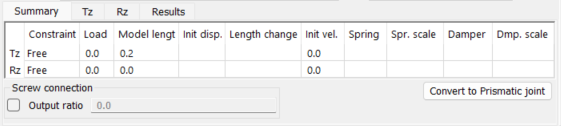
\includegraphics[trim=255 10 2 15,clip,width=0.34\textwidth]{\ReferenceImg/prp/cylindric-joint-1}}
  \end{picture}
\end{wrapfigure}

You can easily convert a Cylindric joint to a
\protect\hyperlink{prismatic-joint}{\sl Prismatic joint} by using the
\textbf{Convert to Prismatic joint} button in {\sl Summary} tab of the
Cylindric joint Property Editor panel (shown to the right).
The {\sl Tz} properties will then be transferred to the Prismatic joint,
whereas the {\sl Rz} properties of course will be lost.

Similaraly, a Prismatic joint will have a
\textbf{Convert to Cylindric joint} button in its {\sl Summary} tab,
which will add an (initially {\sl Free}) {\sl Rz} DOF.


\subsubsection{Cam joint}

\IconTextFirst{camJoint}{
  A cam joint has six unconstrained DOFs that allow the slave triad (a.k.a.
  the {\sl follower}) to move over a curved surface (the {\sl cam surface}).
  The cam surface is defined by a curve consisting of three-point circular arcs.
  Each arc is defined by the location of three master triads,
  also called the {\sl cam triads}.
  A cam joint must consist of one follower triad and at least three cam triads.
  See also the \FedemTGuide{Section 6.3.3, "Cam joint"}.}

It is recommended to use at least one arc segment per quarter of a circle
to make the solution more stable.
This means you will need at least eight master/cam triads for a complete circle.

\Tip{You can use the same cam triads in several different cam joints, making it
  possible to constrain several follower triads to the same cam surface.}

\noindent
\begin{minipage}{0.67\textwidth}
  \raggedright
  An example cam joint is shown to the right.
  %
  \vskip2mm
  \begin{bulletlist}
    \setlength\itemsep{1mm}
  \item Slave/follower triad
  \item Master/cam triads
    (represented by the sets of $X$, $Y$ and $Z$-axes extending from the curve)
  \item Cam curve (represented by the curve)
  \end{bulletlist}
\end{minipage}% <--- the % is needed here to kill off spurious spacing
\hfill\begin{minipage}{0.22\textwidth}
  \begin{picture}(75,75)
    \put(0,-20){\includegraphics[width=\textwidth]{Figures/cam joint symbol}}
    \put(22,65){\Bullet{1}}
    \put(-7,33){\Bullet{2}}
    \put(45,-12){\Bullet{3}}
  \end{picture}
\end{minipage}

\subsubsection{\sl\textbf{Creating cam joints}}

The cam curve is defined by circular arcs and straight lines. Each three-point
arc is defined by three triads. If the triads are located on a straight line,
a straight line will be defined (circular arc with zero curvature).

To create a cam joint, complete the following steps:

\begin{enumerate}
\item
  Click the cam joint icon.
\item
  Select a position for a new follower triad, or select an existing triad.
\item
  Confirm by pressing Done. If an existing triad was selected,
  this triad will become the follower triad, otherwise a new triad is created.
\item
  Select a position for the first master, or select an existing triad.
  You can also select an existing cam curve.
\item
  Confirm by pressing Done. If an existing triad was selected,
  this triad will become the first cam triad, otherwise a new triad is created.
  If an existing cam curve was selected, the new cam joint is complete,
  and the selected cam surface will be used by the new follower triad.
\item
  Repeat steps 4 and 5 until a sufficient number of masters has been
  added. As you add triads, they will be oriented automatically to have
  sensible orientations related to the cam curve. The $Z$-direction is set
  to point along the cam curve, while the $X$-direction, considered to be
  ``up'', is calculated from the direction going from the master triad
  closest to the follower and to the follower triad.
\item
  To close the cam loop, add the first master triad as the last one.
\item
  Fedem tries to set sensible directions on the master triads created,
  but should any of the directions be inconvenient,
  rotate them using one of the tools to move mechanism elements.
  See \refSection{moving-mechanism-elements}{Moving mechanism elements}.
\end{enumerate}
\vskip\parskip
\begin{minipage}{0.6\textwidth}
  \raggedright
  \begin{itemize}
  \item[9.]
    Define the spring characteristics you need for the contact behavior,
    and assign them to the correct joint variables. Normally, a non-linear
    spring with a stiffness-deflection curve as shown in the picture to
    the right will provide a decent contact behavior when assigned to the
    $X$-translation DOF.
  \end{itemize}
\end{minipage}% <--- the % is needed here to kill off spurious spacing
\hfill\begin{minipage}{0.37\textwidth}
  \includegraphics[width=\textwidth]{Figures/4-3-4-CamJointStiffness}
\end{minipage}

\subsubsection{\sl\textbf{Local coordinate system}}

The local coordinate system for a cam joint has its origin on the cam
curve at a point calculated as the closest point to the follower; this
point is referred to as the {\sl contact point}. The local $X$-axis is
then defined to be perpendicular to the cam surface and the $Z$-axis
tangential to the cam curve. The orientation of the local coordinate
axes depends thus on the location of the contact point along the cam curve.

\subsubsection{\sl\textbf{Cam joint variables}}

Cam joints display all the six DOFs as joint variables in the Property
Editor panel, but have some restrictions on the {\sl Constraint Type}
setting that is unique for cam joints.
The only legal settings are {\sl Free} and {\sl Spring-Damper}.
The {\sl Fixed} and {\sl Prescribed} settings are not available because
the cam joint uses a different formulation than the other joints.

The three main joint variables, defined in the $X$-, $Y$- and $Z$-directions
of the cam joint's local coordinate system, are:

\begin{itemize}
\item{\sl X-position} :
  The distance from the contact point to the follower in the
  direction normal to the cam surface (the ``thickness'' direction).

\EnumTip{If no stiffness is assigned to the $X$-translation DOF,
  the whole cam joint will be completely ignored by the Dynamics Solver.
  This might be used as a simple tool to toggle a cam joint
  on and off during testing and modeling of complex models.
  The solver issues a warning when the $X$-translation spring is missing.}

\item{\sl Y-position} : The distance from the contact point to the follower
  in the direction tangential to the cam surface and normal to the cam curve
  (``width'' direction).

\item{\sl Z-position} : The distance along the cam curve from the first
  cam triad to the contact point (the slider variable).
\end{itemize}

You are also allowed to Spring-Damper constrain the rotational DOFs of
the cam joint. Such rotational stiffness/damping might be beneficial as
a stabilization tool in some cases.

\Warning{The rotational DOFs in a Cam joint are not suited for representing
  large rotations. However, this affects the solution only when
  some of these DOFs are Spring-Damper constrained.
  Therefore, when Spring-Damper constraining the rotational DOFs,
  you must ensure that the added stiffness is high enough to keep the rotations
  small, typically $R_x < 0.3$, $R_y < 0.6$ and $R_z < 3.0$ radians.
  If not, the solution will probably diverge.}

The initial values of the cam joint variables are interpreted differently
compared with the other joint types.
The {\sl Length/Angle in model} quantity is always zero for all variables,
regardless of the modeling position of the follower.
For the $T_x$ and $T_y$ DOFs, this means that the deflection is always
calculated as the distance from the contact point to the follower in the local
$X$- and $Y$-directions, respectively.
However, for the $T_z$, $R_x$, $R_y$ and $R_z$ DOFs, the deflection is measured
relative to the modeling position of the follower.
The stress free length/angle of any springs associated with these DOFs are then
also defined relative to these initial positions.

\Warning{If the follower is not within the contact domain of the cam joint
  (see \protect\hyperlink{cam-thickness-and-width}
  {\sl"Cam thickness and width as contact domain"} below)
  at the beginning of the first time step, the rotational springs as well as
  the slider spring, if any, are ignored throughout the simulation.
  This happens because the stress free length of these springs then are
  undefined. A warning is issued from the dynamics solver if this occurs.}

\subsubsection{\sl\textbf{Cam friction}}

The friction parameters for cam joints are the same as those for
prismatic joints with the exception of the equivalent force,
which is the sum of the $X$-spring and $X$-damper force in the cam joint.
The friction state depends on the slider variable only.

\SubSubSection{\sl\textbf{Cam thickness and width as contact domain}}
              {cam-thickness-and-width}

\begin{wrapfigure}[3]{r}{0.4\textwidth}
  \vspace{-4.5mm}
  \includegraphics[width=0.4\textwidth]{Figures/4-JointPropCamFields}
\end{wrapfigure}

The thickness and width parameters shown in the Property Editor panel
define a rectangular domain in the $XY$-plane of the local coordinate system,
and is used to determine whether it is necessary to test if the follower
is in contact or not.
The springs and dampers associated with joint variables are activated only when
the follower is located within the distance {\sl Thickness}/2 from the cam curve
in the local $X$-direction and within the distance {\sl Width}/2 in the local
$Y$-direction. Use of a reasonable thickness is of great importance
to ensure that the contact springs are attached to the correct cam segment
(a cam segment is the part of a cam curve between two triads).
One should avoid having the cam thickness so large that two cam segment have
overlapping contact domains.

\Caution{When assigning highly non-linear spring characteristics
  to the cam joint variables to model contact behavior, it is often necessary to
  assign some associated damping to reduce fictitious oscillations due to sudden
  activation and deactivation of contact spring forces.
  A constant damping coefficient is then sufficient as long as the follower
  is within the contact domain throughout the simulation.
  However, if the follower enters the contact domain once or several times
  during the simulation, numerical instabilities may occur due to the sudden
  activation of the joint variable dampers, because they are active
  only when the follower is within the contact domain.
  To avoid this, it might be necessary to scale the damping coefficient
  with a function (see \refSection{damper-properties}{Damper properties}),
  that varies gradually from zero as the follower enters the contact domain,
  to one as the contact stiffness is activated.}

\subsubsection{\sl\textbf{Radial contact springs}}

By enabling the {\sl Use radial stiffness} toggle, the springs
associated with the $X$- and $Y$-variables are referred to local polar
coordinates in the $XY$-plane instead. Thus, the $X$-coordinate is then the
radial distance from the cam curve to the follower, and the $Y$-coordinate
is the angle between the local Cartesian $X$-axis and the axis extending
from the contact point through the follower. The contact domain will
consequently be a circular cylinder instead of a rectangular one, and
the {\sl Thickness} and {\sl Width} parameters above will now define
the radial and the angular (in degrees) extension of the contact domain.
This can be used to simulate contact in pipes, etc.

\Note{The {\rm Use radial stiffness} toggle does not affect the dampers (if any)
  that are assigned to the joint variables. They are still applied in the local
  Cartesian coordinate system. It is therefore advisable to apply the same
  damping characteristics to the $X$- and $Y$-variables when using radial
  stiffness, to ensure a proper damping behavior in the cam joint.}

\subsubsection{\sl\textbf{Cam with spherical or cylindrical follower}}

Often the follower in a cam joint should have a spherical or cylindrical
shape. Below, we describe how such behaviour can be modelled.

The radius of the sphere or cylinder must be entered as an
{\sl Initial stress free length} for the spring in the $X$-translation DOF
(see \refSection{spring-properties}{Spring properties}).
A normal contact stiffness function can then be used.
The {\sl Thickness} of the cam must also be set to a value greater than
the roller radius in this case.

This will work as expected as long as the follower never is in contact
with the cam curve at more than one location simultaneously.
This means that the follower can not pass the inside of a v-shaped cam curve,
or curve segments that have a radius equal to, or less than the roller radius.
By trying to do so, the numerical simulation will normally fail to converge
when two simultaneous contact locations would be expected.

If the cam curve to be modeled has this kind of features, you will need to model
the different parts of the contact curve as {\sl separate cam joints} instead,
and re-use the same triad as follower in all those cam joints.
You will also have to set them up with the same contact spring
characteristics and {\sl Initial Stress free length}.

\Caution{When using a radius on the follower, even small discontinuities of the
  cam tangent between curve segments might result in a v-shaped curve.
  The v's can cause numerical problems if the follower is on the inside of it.}


\clearpage
%%%%%%%%%%%%%%%%%%%%%%%%%%%%%%%%%%%%%%%%%%%%%%%%%%%%%%%%%%%%%%%%%%%%%%%%%%%%%%%%
\Section{Joint pair constraints}{joint-pair-constraints}

Joint pairs available in Fedem include Gear and Rack-and-Pinion objects.
In addition, you can create general couplings using {\sl Generic DB} objects.


\SubSection{Gear}{gear}

\IconTextFirst{gear}{
  A gear is a rotational constraint between two revolute joints.
  The gear constrains the two joints to rotate at a given transmission ratio.}

\begin{wrapfigure}{r}{0.5\textwidth}
  \vspace{-5mm}
  \includegraphics[width=0.4\textwidth]{Figures/4-GearSymbol.png}
\end{wrapfigure}

\subsubsection{Gear symbol}

The gear symbol (shown at right) is displayed in the {\sl Modeler} view
as a line between two revolute joints.

\begin{wrapfigure}{r}{0.5\textwidth}
  \includegraphics[width=0.5\textwidth]{Figures/4-TransmissionRatio}
\end{wrapfigure}

\subsubsection{Transmission ratio}

You can specify the gear transmission ratio (dimensionless rate) in the
Property Editor panel (shown at right). For information about the gear
transmission ratio, see the \FedemTGuide{Section 6.4.1, "Gear joint"}.


\SubSection{Rack-and-Pinion}{rack-and-pinion}

\IconTextFirst{rack-and-pinion}{
  Rack-and-Pinion is a constraint between a prismatic and a revolute joint.
  The complete system is considered a five-DOF joint that constrains only
  a rotational input displacement to a translational output displacement.
  The joint has a transmission ratio similar to that of gears.}

\subsubsection{Rack-and-Pinion symbol}

\noindent
\begin{minipage}{0.6\textwidth}
  \raggedright
  The Rack-and-Pinion symbol (shown at right) is displayed in the
  {\sl Modeler} view as a line between a prismatic joint and a revolute
  joint.
\end{minipage}% <--- the % is needed here to kill off  spurious spacing
\begin{minipage}{0.4\textwidth}
  \raggedleft
  \includegraphics[scale=0.25]{Figures/4-rack-and-pinion-symbol}
\end{minipage}

\subsubsection{Transmission ratio}

\begin{minipage}{\textwidth}
You can specify the transmission ratio (dimensionless rate) for a
Rack-and-Pinion constraint in the Property Editor panel
(see \refSection{gear}{Gear}).
\end{minipage}

\clearpage
\SubSection{General joint pair constraints}{general-joint-pair-constraints}

In addition to the specific cases
\protect\hyperlink{gear}{\sl Gear} and
\protect\hyperlink{rack-and-pinion}{\sl Rack-and-Pinion},
any other joint pair constraint can be modeled using a Generic database object.
See \refSection{generic-database-objects}{Generic database objects}
on how to create and manipulate such objects.

\begin{wrapfigure}[8]{r}{0.4\textwidth}
  \vspace{-8mm}
  \includegraphics[width=0.28\textwidth]{Figures/4-gen-joint-pair-constr}
\end{wrapfigure}

A joint pair constraint is created by using the {\sl Type} keyword
{\tt HIGHER\_PAIR} and by specifying the two joints and DOFs to be coupled
in the {\sl Definition} field, as in the example shown to the right.
The transmission ratio between the two joint DOFs is specified using the
{\tt coeff} keyword in the {\sl Definition} field, as shown.

\Note{The ID numbers used in the joint identification are their base ID.
  (You can find the base ID of an object using the Object Browser, see
  \refSection{object-browser}{Object Browser}.)}


%%%%%%%%%%%%%%%%%%%%%%%%%%%%%%%%%%%%%%%%%%%%%%%%%%%%%%%%%%%%%%%%%%%%%%%%%%%%%%%%
\Section{Frictions}{frictions}

Joint friction is based on the forces, moments, and velocity in a joint.
These forces and moments give an equivalent load,
which is the basis for computing the friction force.
For a detailed description of friction behavior,
see the \FedemTGuide{Section 6.5, "Joint friction"}.

\begin{wrapfigure}[8]{r}{0.55\textwidth}
  \vspace{-4mm}
  \includegraphics[width=0.5\textwidth]{Figures/4-Friction}
\end{wrapfigure}

You can create a friction by right-clicking an empty space in the Model
Manager {\sl Objects} list, selecting \textbf{Create}, \textbf{Friction} and
then the desired friction type. You can also access this command from the
{\sl Mechanism} menu in the main window.

Frictions are managed in the Model Manager {\sl Objects} list.
If you have created frictions, you can expand the {\sl Friction} group to see
a list of the frictions in your model.
Selecting a friction from the {\sl Objects} list displays the friction
properties in the Property Editor panel. Each type of friction has a different
image and parameters associated with it. The figure below shows the
Property Editor panel with prismatic joint friction selected.

\clearpage
\begin{figure}[H]
  \includegraphics[width=\textwidth]{Figures/friction properties panel}
\end{figure}

To edit the friction, enter new values for each of the friction parameters
listed in the Property Editor panel.
See the \FedemTGuide{Section 6.6, "Joint friction"}
for a description of friction parameters.

\Tip{To associate the friction with the appropriate joint, select the joint
and edit its friction properties in the Property Editor panel.}


%%%%%%%%%%%%%%%%%%%%%%%%%%%%%%%%%%%%%%%%%%%%%%%%%%%%%%%%%%%%%%%%%%%%%%%%%%%%%%%%
\Section{Springs and Dampers}{springs-and-dampers}

There are two types of springs and dampers in Fedem: Axial- and joint springs
and dampers. An axial spring or damper applies relative forces between two
triads along the direction between the triads. Joint springs and dampers are
integrated in the joint, and act on the joint triads along one of the joints
unconstrained DOFs (see \refSection{joint-variables}{Joint variables}).

Both types of spring and dampers have the same options, and they will be
described below. The joint springs and dampers are accessed through the
Property Editor panel of the joint they are used in
(see \refSection{joint-properties}{Joint properties})
while the axial springs and dampers are separate items with 3D symbols
and their own Property Editor panels.


\SubSection{Spring properties}{spring-properties}

The spring properties (shown below) consist of the following options:

\begin{figure}[H]
  \begin{picture}(343,72)
    \put(0,0){\includegraphics[width=\textwidth]{Figures/4-springProp}}
    \put(140,54){\Bullet{1}}
    \put(140,35){\Bullet{2}}
    \put(130,7){\Bullet{3}}
    \put(290,50){\Bullet{4}}
    \put(290,35){\Bullet{5}}
  \end{picture}
\end{figure}

\subsubsection{Stress free length/angle control}

This group of options concerns the calculation of spring deflection. The
deflection is defined as positive when it is increasing the spring length.

\begin{bulletlist}
\item{\sl Length/Angle in model} --
  The current distance (for translation) or angle (for rotation) measured in
  the model as you have made it. For joint springs, this is the measured value
  of the joint DOF that the spring acts on. For axial springs,
  it is the distance between the two triads.

\item{\sl Initial stress free length/angle, Initial deflection} --
  These radio buttons and fields work together allowing you to introduce
  pre-stress in the spring, by setting an initial stress free length/angle
  different from the {\sl Length/Angle in model}.
  You can chose to enter this property either as an absolute value, using the
  {\sl Initial stress free length/angle} option, or relative to the
  {\sl Length/angle in model} by selecting the {\sl Initial deflection} option.

\EnumCaution{If you introduce a spring pre-stress in this manner,
  it will be accounted for in the very first iteration of the dynamics
  simulation and thus lead to a dynamic shock effect.
  However, when initial \refSection{static-equilibrium-analysis}
  {Static equilibrium analysis} is switched on, the pre-stress force
  is taken as a pure static load and the transient shock should be avoided.}

\EnumNote{The initial deflection is positive when it increases
  the spring length/angle.}

\item{\sl Stress free length/angle change} --
  You can select a function to change the stress free length/angle of the spring
  during the simulation (see \refSection{functions}{Functions}).
  The value of the function will be used as an addition to the initial stress
  free length/angle defined above.

\EnumTip{You can introduce motion into your system by using this option to
  change the length of a very stiff spring. However, an alternative and probably
  better way (for joint variables) is to use the Prescribed constraint type
  (see \refSubSection{joint-variable-properties}{Joint variable properties}
  {joint-properties}).
  In that case the stiff spring is avoided and the DOF is eliminated as an
  unknown from the system of equations.
  In most cases, this yields a more stable solution.}
\end{bulletlist}


\subsubsection{Spring properties}

This group of options controls how the deflection is evaluated to produce the
spring force or torque. The spring can be either a linear spring with a constant
stiffness, or a non-linear spring with a non-linear relationship between the
deflection and the force/torque or the stiffness.

The spring force/torque is reckoned to be positive when it is working in
the opposite direction of the increasing spring length/angle.

\begin{bulletlist}
  \setcounter{enumi}{3}
\item
  In this field you can enter a constant spring stiffness or select a
  defined spring characteristic from the pull-down menu.
\item{\sl Scale} --
  The spring force or torque can be scaled by a function.
  This can for instance be used to switch the spring on and off during
  the simulation. When no function is selected the scale is set to 1.0.
\end{bulletlist}


\SubSection{Damper properties}{damper-properties}

\begin{wrapfigure}{r}{0.35\textwidth}
  \begin{picture}(102,50)
    \put(0,0){\includegraphics[width=0.3\textwidth]{Figures/4-DamperProperty}}
    \put(60,30){\Bullet{1}}
    \put(60,16){\Bullet{2}}
    \put(75,4){\Bullet{3}}
  \end{picture}
\end{wrapfigure}

This group of options controls the evaluation of a damper's force or torque
from its velocity. Both linear and non-linear dampers are allowed.
A linear damper uses a constant damping coefficient.
A non-linear one uses a function to control how the damper force or coefficient
depends on its velocity.

\begin{bulletlist}
\item
  In this field a constant damping coefficient can be entered, or you
  can select a damper characteristic from the pull-down menu.
\item{\sl Scale} --
  The damper force or torque can be scaled by a function.
  This can for instance be used to switch the damper on and off during
  the simulation. When no function is selected the scale is set to 1.0.

\EnumNote{In Fedem version 2.5 or lower, non-linear dampers were modeled using
  a function to change the damper coefficient.
  When opening such models in the curent version, those dampers are converted
  by setting the damper functions as scale functions,
  and the coefficient to 1.0.}

\item{\sl Use deformational velocity} --
  This option is available only if the damper is acting together with a spring
  with a forced change in its stress free length. The option enables the usage
  of the deformational velocity of the connected spring, when evaluating the
  damper. The deformational velocity is the spring velocity without the
  velocity component coming from a forced change in the stress free length.

\EnumNote{The use deformational velocity toggle is not visible for axial dampers
  unless there is a parallel axial spring connected to the same triads.}
\end{bulletlist}


\SubSection{Axial spring symbol}{axial-spring-symbol}

\vskip\parskip
\IconTextFigure{spring}{
  The symbol for an axial spring is displayed in the {\sl Modeler} view as shown
  to the right.
  \vspace{1mm}
  \begin{bulletlist}
    \item First triad
    \item Axial spring
    \item Second triad
  \end{bulletlist}}{Figures/SpringSymbol}


\SubSection{Axial damper symbol}{axial-damper-symbol}

\vskip\parskip
\IconTextFigure{damper}{
  The symbol for an axial damper is displayed in the {\sl Modeler} view as shown
  to the right.
  \vspace{1mm}
  \begin{bulletlist}
    \item First triad
    \item Axial damper
    \item Second triad
  \end{bulletlist}}{Figures/DamperSymbol}


\SubSection{Spring and damper characteristics}
{spring-and-damper-characteristics}

Non-linear springs and dampers are defined by creating a spring or
damper characteristics objects. There are four basic types of
characteristics available both for springs and dampers. The differences
between them are whether they define a rotational or translational
behavior, and whether they define a stiffness/damping coefficient curve
or a force/torque curve. In addition, there are two types of advanced
spring characteristics available (for translational and rotational
springs, respectively), see \refSection{advanced-spring-characteristics}
{Advanced spring characteristics}.

\SubSubSection{Spring characteristics}{spring-characteristics}

The four basic spring characteristics types are:

\begin{itemize} \setlength\itemsep{0.2em}
  \item Force - Translation
  \item Torque - Rotation
  \item Stiffness - Translation
  \item Stiffness - Rotation
  \end{itemize}

\subsubsection{\sl\textbf{Force-Translation/Torque-Translation}}

These characteristics describe the relationship between displacement
and spring force/torque directly. The spring stiffness is then computed as
the derivative of the provided curve.

$$
  k(\Delta) = \frac{dF(\Delta)}{d(\Delta)}
$$

\subsubsection{\sl\textbf{Stiffness-Translation/Stiffness-Rotation}}

These characteristics describe the relationship between the displacement
and the spring stiffness directly. The spring force/torque is then computed as
the integral of the provided curve from 0 to the current deflection

$$
  F = \int\limits_0^\Delta k(x) dx
$$

The definition of the curves used can be done using one of the following
function shape types (see \refSection{function-types}{Function Types}):

\begin{itemize}
\item Polyline and Polyline from file
\item Constant
\item Linear
\item Ramp and Limited Ramp
\end{itemize}

A more detailed description of the spring characteristics can be found in the
\FedemTGuide{Section 5.1, "Spring Elements"}.

\subsubsection{Damper characteristics}

The four types of damper characteristics are:

\begin{itemize}
\item Force - Velocity
\item Torque - Angular velocity
\item Coefficient - Velocity
\item Coefficient - Angular velocity
\end{itemize}

\subsubsection{\sl\textbf{Force-Velocity/Torque Angular velocity}}

These characteristics describe the relationship between the damper velocity
and damper force/torque directly.
If a function $g(v)$ is used, the damper force is $F(v)=g(v)$ for all $v$.
The damping coefficient is computed as the derivative $g'(v)$.
A regular damper will have a $g(v)$ that is positive for positive $v$,
and vice versa.

\subsubsection{\sl\textbf{Coefficient-velocity/Coefficient-Angular velocity}}

These characteristics are interpreted as the derivative of the force/torque-
velocity function with respect to $v$. The damper force at a specific $v$ is
thus $F(v)=\int_0^vg(w)dw$ for a given function $g(v)$,
and the damping coefficient is the function value directly. A regular damper
will have a coefficient-velocity function with positive values only.

The damper characteristics can be defined using the same function types
as for the spring characteristics (see
\protect\hyperlink{spring-characteristics}{\sl"Spring characteristics"} above).
A more detailed description of the damper characteristics can be found
in the \FedemTGuide{Section 5.2, "Damping Elements"}.

\SubSubSection{Creating spring and damper characteristics}{creating-spr-dmp}

To create a spring or damper characteristic, right click in the Model Manager
{\sl Objects} list, and select \textbf{Create} $\rightarrow$
\textbf{Spring/Damper characteristic} and then the type you want from the menus
shown below:

\begin{figure}[H]
  \includegraphics[height=0.2\textwidth]{Figures/4-SpringCharacteristics} \hfill
  \includegraphics[height=0.2\textwidth]{Figures/4-DamperCharacteristics}
\end{figure}

The characteristics you have created, will be displayed in the proper
pull-down menus in the spring and damper Property Editor panels. Only
those of correct type will be listed, to avoid using characteristics
defined for rotation in translational DOFs and vice versa.


\SubSection{Advanced spring characteristics}{advanced-spring-characteristics}

In addition to the basic spring characteristics types described above,
there are also some more advanced characteristics available with further
options for defining the non-linear behavior of a spring. The Property
Editor panel for the advanced spring characteristics is displayed below.

\begin{figure}[H]
  \begin{picture}(343,112)
    \put(0,0){\includegraphics[width=\textwidth]{Figures/4-AdvancedSpringCharacteristics}}
    \put(60,94){\Bullet{1}}
    \put(60,69){\Bullet{2}}
    \put(60,34){\Bullet{3}}
  \end{picture}
\end{figure}

\begin{bulletlist}
\item{\sl Spring function} --
  In this field you may either enter a constant spring stiffness,
  or select an existing basic spring characteristics function from the
  pull-down menu.

\item{\sl Failure criterions} --
  Failure of the spring can be defined through the maximum and minimum forces
  and deflections. You can enable all four criteria, and whichever failure
  criterion is satisfied first will switch the spring (permanently) off
  (i.e., both spring force and stiffness vanishes).
  \begin{itemize}
  \subitem{\sl Max Deflection} :
    Spring is active until its deflection becomes greater than this value.
  \subitem{\sl Min Deflection} :
    Spring is active until its deflection becomes less than this value.
  \subitem{\sl Max Force} :
    Spring is active until force becomes greater than this value.
  \subitem{\sl Min Force} :
    Spring is active until force becomes less than this value.
  \end{itemize}

\item{\sl Yield criterion} --
  Hysteresis behavior and/or permanent deflection after unloading can be
  introduced in springs by this options. The yield criterion will limit the
  force of the spring to the specified maximum and minimum forces.
  When the spring force reaches any of these limits, the spring stiffness
  vanishes and any further deflection of the spring is defined as the
  {\sl yield deflection}.
  \begin{itemize}
  \subitem{\sl Max Yield Force} :
    Spring force is always less than this value if this option is enabled.
  \subitem{\sl Min Yield Force} :
    Spring force is always greater than this value if this is option is enabled.
  \subitem {\sl Max Yield Deflection} :
    If the yield deflection exceeds this value (either on tension or
    compression) the spring is switched permanently off.
  \end{itemize}
\end{bulletlist}

\Note{The {\rm Max Yield Force} and {\rm Min Yield Force} can also be defined
  through functions giving the spring variable yield limits. This can be used to
  model clutch-like behaviors in a spring coupling, where you can smoothly
  (or abruptly) engage/disengage the motion coupling.}

To define a non-linear spring with sudden failure and/or yield limits,
you have to define the non-linear elastic force-deflection (or
stiffness-deflection) curve first, through the {\sl Spring characteristics} menu
(see \protect\hyperlink{creating-spr-dmp}
{\sl"Creating spring and damper characteristics"} above).
Then you create an {\sl Advanced Spring Characteristic} via the same
menu, select the newly created Spring Characteristic in the
{\sl Spring function} pull-down menu, and then add the failure/yield criteria.
The advanced spring characteristic is then available for selection in the
\protect\hyperlink{spring-properties}{\sl Spring properties} field
of the Spring objects.


\Section{Loads}{loads}

\vskip\parskip
\IconsText{force}{torque}{
  Two types of loads can be applied to triads or parts: forces and torques.
  Both types are applied as point-force vectors on FE nodes. These loads can be
  used to introduce motion into your mechanism. During simulation, the magnitude
  of forces and torques can be constant or controlled by functions
  (see \refSection{functions}{Functions}). When creating them,
  it is possible to add a load directly to an existing triad or to an FE node.}


\SubSection{Load symbols}{load-symbols}

\noindent
\begin{minipage}{0.45\textwidth}
  The symbols for forces and torques are displayed in the {\sl Modeler} view
  as shown to the right.
\end{minipage}%
\hfill\begin{minipage}{0.5\textwidth}
  \begin{picture}(135,80)
    \put(0,0){\includegraphics[width=20mm]{Figures/4-LoadForceSymbol}}
    \put(80,-7){\includegraphics[width=20mm]{Figures/4-LoadMomentSymbol}}
    \put(15,80){Force}
    \put(92,80){Torque}
  \end{picture}
\end{minipage}


\SubSection{Load properties}{load-properties}

The magnitude and direction of a force/torque vector can be edited in the
Property Editor panel (shown below).
Select the force or torque to show its properties.

\begin{figure}[H]
  \begin{picture}(243,104)
    \put(0,0){\includegraphics[width=\textwidth]{Figures/force property editor panel}}
    \put(35,82){\Bullet{1}}
    \put(50,63){\Bullet{2}}
    \put(150,85){\Bullet{3}}
    \put(102,55){\Bullet{4}}
    \put(102,33){\Bullet{5}}
    \put(-50,-72){\includegraphics[width=7mm]{Figures/mouse}}
    \put(-50,-185){\includegraphics[width=7mm]{Figures/eyes}}
  \end{picture}
\end{figure}

\begin{bulletlist}
  \setlength\itemsep{1mm}

\item{\sl Magnitude} --
  To change the load magnitude, enter a constant value or select one from the
  list of functions in your model (see \refSection{functions}{Functions}).

\item{\sl Load Target Point} --
  The point is given in either global or local coordinates.
  You can also select a new target point using the \textbf{Mouse} button
  (see \refSection{target-point}{Target point} below).

\item{\sl Direction} --
  The {\sl From} and {\sl To} options allow you to edit the orientation of the
  load vector (see \refSection{direction}{Direction} below).

\item
  You can select a new point for the {\sl Load Target Point}, or {\sl From}
  or {\sl To Directions} using the \textbf{Mouse} buttons
 (then select a new point in the {\sl Modeler} view).

\item
  You can click and hold down any of the \textbf{View} buttons in the Property
  Editor panel to highlight the corresponding point in the {\sl Modeler} view.
\end{bulletlist}


\SubSection{Target point}{target-point}

\IconTextFirst{../mouse}{
  To specify a new target point, click the \textbf{Mouse} button and use the
  cursor to select a part in the {\sl Modeler} view.
  If the target point does not coincide with an FE node, the target point will
  snap to the closest node. Press \textbf{Done} to confirm the selection.
  A triad is created at that position.}

\SubSection{Direction}{direction}

\RightFigure{4-Direction-text}{
  The direction of the input load vector can be specified by two points moving
  together with the selected parts, or by two fixed points given
  in global coordinates. The direction is given by the vector pointing
  from the {\sl From} point to the {\sl To} point (shown at right).}


%%%%%%%%%%%%%%%%%%%%%%%%%%%%%%%%%%%%%%%%%%%%%%%%%%%%%%%%%%%%%%%%%%%%%%%%%%%%%%%%
\Section{Functions}{functions}

\IconTextFirst{function}{
  Functions can be used to control the magnitude of loads,
  the length of springs, prescribed motion in joints, etc.
  The function defines one input variable (except for functions of type
  \protect\hyperlink{math-expression}{\sl Math Expression}, which may
  have up to four input variables) and a function shape that is used to
  transform the input value(s) into the output value of the function, The
  output will thus change during the simulation depending on the
  variations in its input value(s).}

The input value can be a system variable measured by a sensor, the
output of a control system, the output of a different function, or
simply the simulation time. The function shape can be defined in several
different ways, and uses a common way of defining function shapes across
different objects needing to do so.

Road elevations, Control inputs, Control outputs, Spring and Damper
characteristics are all examples of objects using a similar way of
defining function-like relationships. The description found here is thus
valid for several other objects as well.


\SubSection{Creating a function}{creating-a-function}

\RightFigure{4-Function}{
  You create a function by right-clicking an empty space in the Model Manager
  {\sl Objects} list, selecting \textbf{Create} and then \textbf{Function}.
  You can also access the command from the \textbf{Mechanism} menu
  in the main window.}

\RightFigure{4-FunctionModelManager}{
  The new Function is automatically selected, and its properties are shown
  in the Property Editor panel. It will also be added to the list of Functions
  maintained in the Model Manager {\sl Objects} list (shown at right).}

\clearpage


\SubSection{Function properties}{function-properties}

When a function is selected in the {\sl Objects} list, its properties are
displayed in the Property Editor panel (shown below) which is divided in three
parts. The left part contains fields for defining the function type and
argument and the middle part contains a list of parameters associated with the
chosen function type. The right part contains two tabs; one for displaying an
image explaining the function definition and another with options for previewing
the function in a graph.

\begin{figure}[H]
  \begin{picture}(243,95)
    \put(0,0){\includegraphics[width=\textwidth]{Figures/4-FunctionProperties}}
    \put(50,83){\Bullet{1}}
    \put(40,58){\Bullet{2}}
    \put(103,49){\Bullet{3}}
    \put(145,83){\Bullet{4}}
    \put(245,90){\Bullet{5}}
    \put(285,90){\Bullet{6}}
  \end{picture}
\end{figure}

\begin{bulletlist}
\item{\sl Function Type} -- You can
  change the function type by selecting the new type from the pull-down menu.
  The parameters and the help image shown in the panel are updated to reflect
  the new type.

\item{\sl Argument} --
  You can select any of the objects in your model that
  already is used as an argument by this or another function; namely
  those having a sensor attached, from the pull-down menu. When an object
  has been selected, specify which
  quantity you want to access on that object by selecting from the
  {\sl DOF} and {\sl Var} pull-down menus.

\item The selection button -- By pressing this button
  you can select any object in your model to use as argument.
  When the button is pressed, the Guide panel will prompt you to select an
  object. Do so and press \textbf{Done} to accept the selection.
  A sensor will then be created on the selected object which will appear in the
  {\sl Argument} pull-down menu. In addition to physical objects like Triads,
  Joints, etc., you may also select Control output elements and other Functions
  as arguments.

\item{\sl Parameters} --
  This frame contains the user-defined parameters of the selected function type.

\item{\sl Parameter Help} --
  This tab displays a reference picture to easier remember the meaning of
  the different parameters.

\item{\sl Preview} --
  This tab has options to control preview of the function shape
  (see \refSection{preview}{Preview}).
\end{bulletlist}


\SubSection{Preview}{preview}

\begin{wrapfigure}[9]{r}{0.38\textwidth}
  \vspace{-4mm}
  \includegraphics[width=0.37\textwidth]{Figures/4-FunctionPreviewTab}
\end{wrapfigure}

To get an impression of the function shape you may preview it as a curve in
a graph. Specify the argument {\sl Domain} and {\sl Increment} in the
{\sl Preview} tab of the Property Editor panel, then push the
\textbf{Show} button to plot. A preview graph containing the preview
curve is then created and displayed. The displayed curve is updated
automatically when changing any of the function properties.

Most functions have the option to set the preview increment automatically. This
is enabled by default, but can be disabled by toggling the {\sl Auto} toggle.

The created graph and curve is automatically added to the Model Manager
Results list and may be handled like any regular graph and curve. (Refer
to \refSection{postprocessing-environment}{Postprocessing environment}
and \refSection{graphs}{Graphs}.)

\Tip{The actual values of a function can also be plotted directly in a Graph
  when you have run a simulation or during a simulation. To enable such
  plotting, you must first specify the Additional Solver Option
  {\tt -allEngineVars} for the Dynamics Solver (see
  \refSection{additional-solver-options}{Additional solver options}) before
  starting the simulation, such that the function values are saved to the
  results database files for the computed time steps.}


\SubSection{Extrapolation}{extrapolation}

\begin{wrapfigure}[7]{r}{0.37\textwidth}
  \vspace{-4mm}
  \includegraphics[width=0.37\textwidth]{Figures/4-FunctionExtrapMenu}
\end{wrapfigure}

For functions defined on a user-specified finite domain, the option to
extrapolate the function outside this domain exists (i.e., functions of type
Polyline, Linear derivative or Spline). The default is no extrapolation (None).

If the {\sl Extrapolation} option is set to Flat the function retains
the end point values when outside its domain. That is:

\begin{itemize}
\item
  For all $\nu < x_1$ the function evaluates to $f(x_1)$.
\item
  For all $\nu > x_n$ the function evaluates to $f(x_n)$.
\end{itemize}

If the {\sl Extrapolation} option is set to Linear the function is
continued along the tangent line of the nearest end point, that is:

\begin{itemize}
\item
  For all $\nu < x_1$ the function evaluates to $f(x_1) + f'(x_1)*(\nu-x_1)$.
\item
  For all $\nu > x_n$ the function evaluates to $f(x_n) + f'(x_n)*(\nu-x_n)$.
\end{itemize}


\SubSection{Function Types}{function-types}

All function types available in Fedem are presented in the following.

\subsubsection{1:1}

This represents the identity function. Its value equals the argument value.

\SubSubSection{Polyline}{polyline-function}

This is linear interpolation between user-specified points $(x_i, y_i)$:

$$
  f(v) = y_i + \frac{v-x_i}{x_{i+1} - x_i}(y_{i+1}-y_i)
  \quad\mbox{with}\quad
  x_i < v \leq x_{i+1} \;\forall\; i\in[1,n]
$$

\begin{wrapfigure}[9]{r}{0.5\textwidth}
  \vspace{-12mm}
  \includegraphics[width=0.48\textwidth]{Figures/4-Polyline_numbers}
\end{wrapfigure}

To add many numbers to a polyline function, copy and paste is feasible.
Copy the numbers from the application where they are present (e.g., a
spreadsheet or a text editor). On Windows-based systems they have to be copied
to the clip board by pressing \textbf{Ctrl+C}. The numbers are then inserted
into the polyline function by clicking the list and pressing \textbf{Ctrl+V}.

Refer to \refSection{extrapolation}{Extrapolation} to learn about the
extrapolation of a polyline function.

\SubSubSection{Polyline from file}{polyline-from-file}

This function is similar to the polyline function except that the points now are
read from a file. The file format can either be single- or multi-channel
ASCII (\File{.asc}, \File{.txt}), DAC (\File{.dac}) or RPCIII time history
(\File{.rsp}, \File{.drv}, \File{.tim}).
For multi-channel ASCII and RPCIII files, the channel to read is chosen by
pressing the select button \textbf{[...]}. As shown below,
additional parameters for scaling and vertical shift of the function may also
be specified in the Property Editor panel of this function type.

\clearpage
\begin{figure}[H]
  \includegraphics[width=\textwidth]{Figures/4-FunctionPolylineFromFile}
\end{figure}

For abscissa value $v$ the returned ordinate $f(v)$ of the polyline from file
function is

$$
  f(v) = \left(y_i + \frac{v-x_i}{x_{i+1} - x_i}(y_{i+1}-y_i)\right)s + k
  \quad\mbox{with}\quad
  x_i < v \leq x_{i+1}, \; \forall\; i\in[1,n]
$$
where $s$ is the {\sl Scale} factor and $k$ is some vertical shift (see below).

This function interpolates linearly between the user-specified points
$(x_i, y_i)$. The interpolated ordinate value is then scaled by the factor $s$,
and shifted by $k$. The vertical shift value $k$ is set to the scalar $\kappa$
entered in the {\sl Additional shift} field.
If the toggle {\sl Shift function to zero out start value} is checked as well,
the start value $x_1$ is also subtracted, so that $k=\kappa-x_1$.

For abscissa values outside the function domain an extrapolated ordinate
is assigned, such that

$$
  \nu < x_1 \Rightarrow f(v)=f(x_1)
  \quad\mbox{and}\quad
  \nu > x_n \Rightarrow f(v)=f(x_n)
$$

\subsubsection{Spline}

\begin{wrapfigure}[6]{r}{0.45\textwidth}
\vspace{-12mm}
  \includegraphics[width=0.42\textwidth]{Figures/4-Spline_numbers}
\end{wrapfigure}

A third-order spline approximation is calculated from a set of user-specified
points $(x_i,y_i),\;i\in[1,n]$, which may be entered in the same way as for
Polyline functions. At least 4 points are required for a Spline function.

Refer to \refSection{extrapolation}{Extrapolation} to learn about the
extrapolation of a Spline function.

\Tip{If you have a \protect\hyperlink{polyline-function}{\sl Polyline} function
  consisting of at least four points, you can change its type into Spline
  without loosing the entered curve point data. This is useful just to see
  how the same set of points appear when they are interpolated with a
  cubic spline basis instead of the piece-wise linear interpolation.
  You can then change back to Polyline again, if you want to retain the linear
  interpolation in the simulation.}

\SubSubSection{Math Expression}{math-expression}

The math expression function type allows a closed form function expression to be
entered as free text. This is the only function type that may have more than one
input variable (function arguments). The function expression is entered in the
Parameters section of the Property Editor panel as shown below.
The \textbf{Apply} button must be pushed to check and register the expression,
whenever it is updated. The number of input variables are also set in the
Property Editor panel (the default is one input variable).

\begin{figure}[H]
  \includegraphics[width=\textwidth]{\ReferenceImg/prp/math-expression-1}
\end{figure}

The following rules apply for  math expression functions:

\begin{itemize}
\item
  The expression must be functions of either one, two, three or four
  variables, and the independent variable must be named $x,y,z$ and $t$.
\item
  The expression may consist of the intrinsic functions and operators listed
  below, along with the independent variables, $\{x,y,z,t\}$.
\item
  Function expressions may be nested, e.g.:
  \begin{itemize}
  \item[--]
    {\tt sin(cos x)} is a valid expression.
  \end{itemize}
\item
  Precedence is set by parentheses in the usual manner. E.g:
  \begin{itemize}
  \item[--]
    {\tt sin(x\^{}2)} -- $x$ is squared before being input to the sine function.
  \item[--]
    {\tt(sin x)\^{}2} -- the value of sine of $x$ is squared.
  \end{itemize}
\item
  The logical operators have a return 0 if {\sl FALSE} and 1 if {\sl TRUE},
  and are used by multiplying them with the function expressions. E.g,
  \begin{itemize}
  \item[--]
    {\tt sin x + (x\textgreater2)*x} equals {\tt sin x} if $x\le2$,
    and {\tt sin x + x} if $x>2$.
  \end{itemize}
\end{itemize}

Below are the available intrinsic functions and operators.
The symbols {\tt a} and {\tt b} may both be numbers, functions or
the independent variable $x$.

\begin{center}
\vspace{0.3cm}
\begin{tabular}{|>{\raggedright} p{0.23\linewidth}| p{0.48\linewidth}|}
  \hline
  \rowcolor[HTML]{EFEFEF}
  Function & Description   \\
  \hline\hline
  {\tt abs a} & absolute value  \\
  \hline
  {\tt a+b} & addition \\
  \hline
  {\tt a-b} & subtraction \\
  \hline
  {\tt a*b} & multiplication \\
  \hline
  {\tt a/b} & division \\
  \hline
  {\tt a\%b} & modulus \\
  \hline
  {\tt a\^{}b} & power \\
  \hline
  {\tt max(a,b)} & Maximum of a and b \\
  \hline
  {\tt min(a,b)} & Minimum of a and b \\
  \hline
  {\tt sqrt(a)} & power \\
  \hline
  {\tt n\#a} & n-th root \\
  \hline
  {\tt sin a} & sine \\
  \hline
  {\tt cos a} & cosine \\
  \hline
  {\tt tan a} & tangent \\
  \hline
  {\tt asin a} & arcsin \\
  \hline
  {\tt acos a} & arccos \\
  \hline
  {\tt atan a} & arctan \\
  \hline
  {\tt ln a} & logarithm, base e \\
  \hline
  {\tt log a} & logarithm, base 10 \\
  \hline
  {\tt exp a} & exponential, e\textsuperscript{a} \\
  \hline
  {\tt aEb} & a*10\textsuperscript{b} \\
  \hline
  {\tt pi} & constant value of $\pi$ \\
\hline\end{tabular}
\end{center}

\clearpage
Available logical operators:

\begin{center}
\vspace{0.3cm}
\begin{tabular}{|>{\raggedright} p{0.23\linewidth}| p{0.48\linewidth}|}
  \hline
  \rowcolor[HTML]{EFEFEF}
  Function & Description   \\
  \hline\hline
  {\tt !a} & not \\
  \hline
  {\tt a $<$ b} & less than  \\
  \hline
  {\tt a $>$ b} & greater than \\
  \hline
  {\tt a $<=$ b} & less than or equal to \\
  \hline
  {\tt a $>=$ b} & greater than or equal to \\
  \hline
  {\tt a $==$ b} & equal to \\
  \hline
  {\tt a $!=$ b} & not equal to \\
  \hline
  {\tt a $||$ b} & or \\
  \hline
  {\tt a $\&\&$ b} & and \\
\hline\end{tabular}
\end{center}

\subsubsection{Constant}

\noindent
\begin{minipage}{0.45\textwidth}
  \includegraphics[width=\textwidth]{Figures/4-Functions_constant}
\end{minipage}%
\hfill\begin{minipage}{0.4\textwidth}
  $$f(v) = C$$
  $C$ - {\sl Constant} (amplitude)
\end{minipage}

\subsubsection{Linear function}

\noindent
\begin{minipage}{0.45\textwidth}
  \includegraphics[width=\textwidth]{Figures/4-Functions_linear}
\end{minipage}%
\hfill\begin{minipage}{0.4\textwidth}
  $$f(v) = kv$$
  $k$ - {\sl Slope}
\end{minipage}

\subsubsection{Step}

\noindent
\begin{minipage}{0.45\textwidth}
  \includegraphics[width=\textwidth]{Figures/4-Functions_step}
\end{minipage}%
\hfill\begin{minipage}{0.5\textwidth}
  $$
    f(v)=\left\{\begin{array}{ll}
      C   &,\; v < v_0 \\
      C+A &,\; v > v_0
    \end{array}\right.
  $$
  $C$ -- offset (start amplitude \\
  $A$ -- amplitude \\
  $v_0$ -- step abscissa value (delay)
\end{minipage}

\subsubsection{Ramp}

\noindent
\begin{minipage}{0.45\textwidth}
  \includegraphics[width=\textwidth]{Figures/4-Functions_ramp}
\end{minipage}%
\hfill\begin{minipage}{0.5\textwidth}
  $$
    f(v)=\left\{\begin{array}{ll}
      C          &, v < v_0 \\
      C+k(v-v_0) &,\; v > v_0
    \end{array}\right.
  $$
  $C$ -- offset (start amplitude) \\
  $A$ -- amplitude \\
  $v_0$ -- step abscissa value (delay)
\end{minipage}

\subsubsection{Limited ramp}

\noindent
\begin{minipage}{0.45\textwidth}
  \includegraphics[width=\textwidth]{Figures/4-Functions_ramp}
\end{minipage}%
\hfill\begin{minipage}{0.5\textwidth}
  $$
    f(v)=\left\{\begin{array}{ll}
      C          &,\; v < v_0 \\
      C+k(v-v_0) &,\; v_0 < v > v_e \\
      C+k(v_e-v) &,\; v > v_e
    \end{array}\right.
  $$
  $C$ -- offset (start amplitude) \\
  $A$ -- amplitude \\
  $v_0$ -- step start abscissa (start) \\
  $v_e$ -- ramp end abscissa (end)
\end{minipage}

\subsubsection{Pulse}

\noindent
\begin{minipage}{0.45\textwidth}
  \includegraphics[width=\textwidth]{Figures/4-Functions-pulse}
\end{minipage}%
\begin{minipage}{0.55\textwidth}
  $$
    f(v)=\left\{\begin{array}{ll}
      C   &,\; v < v_0 - \frac{\delta}{2} \\
      C+A &,\; v_0 - \frac{\delta}{2} < v < v_0 + \frac{\delta}{2} \\
      C   &,\; v > v_0 + \frac{\delta}{2}
    \end{array}\right.
  $$
  $C$ -- offset (displacement) \\
  $A$ -- amplitude \\
  $\delta$ -- width \\
  $v_0$ -- pulse center abscissa value (position)
\end{minipage}

\SubSubSection{Sine}{sine}

\noindent
\begin{minipage}{0.45\textwidth}
  \includegraphics[width=\textwidth]{Figures/4-Functions-sine}
\end{minipage}%
\begin{minipage}{0.55\textwidth}
  $$
    f(v)=\left\{\begin{array}{ll}
      C+A\sin(2\pi(f_0v-\theta))   &,\; v \leq v_e \\
      C+A\sin(2\pi(f_0v_e-\theta)) &,\; v > v_e
    \end{array}\right.
  $$
  $C$ -- offset (displacement \\
  $A$ -- amplitude \\
  $f_0$ -- frequency [Hz] \\
  $\theta$ -- phase shift (fraction of period) \\
  $v_e$ -- end of sinusoidal
\end{minipage}

\Note{If the end value in a sine function is specified less than or equal
  to zero, that is interpreted as infinity.}

\subsubsection{Combined sine}

$$
  f(v)=\left\{\begin{array}{ll}
  C+A_1\sin(2\pi(f_1v-\theta_1)) + A_2\sin(2\pi(f_2v-\theta_2)) &,\; v \leq v_e \\
  C+A_1\sin(2\pi(f_1v_e-\theta_1)) + A_2 sin(2\pi(f_2v_e-\theta_2)) &,\; v > v_e
  \end{array}\right.
$$
\noindent
\begin{minipage}{0.45\textwidth}
  \includegraphics[width=\textwidth]{Figures/4-Functions-combinedSine}
\end{minipage}%
\hfill\begin{minipage}{0.5\textwidth}
  $C$ - offset (displacement) \\
  $A_1, A_2$ -- amplitudes \\
  $f_1, f_2$ -- frequencies [Hz] \\
  $\theta_1, \theta_2$ -- phase shifts (fraction of period) \\
  $v_e$ -- end of sinusoidal
\end{minipage}

\Note{If the end value in a combined sine function is specified less than or
  equal to zero, that is interpreted as infinity.}

\subsubsection{Delay combined sine}

$$
  f(v)=\left\{\begin{array}{ll}
    C+A_1\sin(2\pi(f_1v_0-\theta_1)) + A_2\sin(2\pi(f_2v_0-\theta_2))
    &,\; v \leq v_0 \\
    C+A_1\sin(2\pi(f_1v-\theta_1)) + A_2\sin(2\pi(f_2v-\theta_2))
    &,\; v > v_0
  \end{array}\right.
$$
\noindent
\begin{minipage}{0.45\textwidth}
  \includegraphics[width=\textwidth]{Figures/4-Functions-delayedSine}
\end{minipage}%
\hfill\begin{minipage}{0.5\textwidth}
  $C$ -- offset (displacement) \\
  $A_1, A_2$ -- amplitudes \\
  $f_1, f_2$ -- frequencies [Hz] \\
  $\theta_1, \theta_2$ -- phase shifts (fraction of period) \\
  $v_0$ -- start of sinusoidal
\end{minipage}

\subsubsection{Periodic square pulse}

$$
  f(v)=\left\{\begin{array}{ll}
  C+A,\; \frac{n-1}{f_0}   < v-\theta \leq \frac{2n-1}{2f_0} \\
  C-A,\; \frac{2n-1}{2f_0} < v-\theta \leq \frac{n}{f_0}
  \end{array}\right.,\; n \in 0,1,2..
$$
\noindent
\begin{minipage}{0.45\textwidth}
  \includegraphics[width=\textwidth]{Figures/4-Functions-PeriodicSquarePulse}
\end{minipage}%
\hfill\begin{minipage}{0.5\textwidth}
  $C$ -- offset (displacement) \\
  $A$ -- amplitude \\
  $f_0$ -- frequency [Hz] \\
  $\theta$ -- phase shift)
\end{minipage}

\subsubsection{Linear derivative function}

\noindent
\begin{minipage}{0.45\textwidth}
  \includegraphics[width=\textwidth]{Figures/4-Functions_LinearDerivativeFunction}
  \vspace*{-15mm}
  $$
    f(v)= \int\limits_0^v f'(\tau)d\tau
  $$
\end{minipage}%
\begin{minipage}{0.55\textwidth}
  $$
    f'(v)=\left\{\begin{array}{ll}
    0                      &,\; 0 \leq v < v_1 \\[1mm]
    \frac{v-v_1}{v_2-v_1}   &,\; v_1 \leq v < v_2 \\[1mm]
    1                      &,\; v_2 \leq v < v_3 \\[1mm]
    \frac{v_4-v}{v_4-v_3}   &,\; v_3 \leq v < v_4 \\[1mm]
    0                      &,\; v_4 \leq v < v_5 \\[1mm]
    \frac{v_5-v}{v_6-v_5}   &,\; v_5 \leq v < v_6 \\[1mm]
    -1                     &,\; v_6 \leq v < v_7 \\[1mm]
    \frac{v-v_8}{v_8-v_7}   &,\; v_7 \leq v < v_8 \\[1mm]
    0                      &,\; v_8 \leq v < v_9 \\[1mm]
    \frac{v-v_9}{v_{10}-v_9} &,\; v_9 \leq v < v_{10}
  \end{array}\right.
  $$
\end{minipage}

To add many numbers to a linear derivative function, copy and paste is feasible.
Copy the numbers from the application where they are present
(e.g., a spreadsheet or a text editor). On Windows-based systems they have to be
copied to the clip board by pressing \textbf{Ctrl+C}.
The numbers are then inserted into the polyline function by clicking the list
and pressing \textbf{Ctrl+V}.

Refer to \refSection{extrapolation}{Extrapolation}
to learn about the extrapolation of a Linear derivative function.

\clearpage
\SubSubSection{Smooth trajectory}{smooth-trajectory}

{\small $$
  f(v)=\left\{\begin{array}{ll}
    0 &,\; t \leq 0 \\[1mm]
    \frac{A_{max}}{4}\left(
      t^2-\frac{1}{2\omega^2}(1-\cos(2\omega t))\right)
      &,\; 0 < t \leq \frac{\pi}{\omega} \\[1mm]
    V_{max}\left(t-\frac{\pi}{2\omega}\right)
      &,\; \frac{\pi}{\omega} < t \leq T-\frac{\pi}{\omega} \\[1mm]
    V_{max}\left(t-\frac{\pi}{\omega}\right) -
      \frac{A_{max}}{4}\left((T-t)^2-\frac{1}{2\omega^2}(1-\cos(2\omega(T-t)))\right)
      \!\!\!\!&,\; T-\frac{t}{\omega} < t \leq T \\[1mm]
    V_{max}\left(t-\frac{\pi}{\omega}\right)
      &,\; t > T
    \end{array}\right.
$$}
where $t=v-v_0$ and $\omega=\frac{\pi}{2}\frac{A_{max}}{V_{max}})$

\noindent
\begin{minipage}{0.45\textwidth}
  \includegraphics[width=\textwidth]{Figures/4-Functions_SmoothTrajectory.png}
\end{minipage}%
\begin{minipage}{0.55\textwidth}
  $v_0$ -- start abscissa value (delay) \\
  $V_{max}$ -- max(f') (maximum velocity) \\
  $A_{max}$ -- max(f'') (maximum acceleration) \\
  $T$ -- length of trajectory
\end{minipage}

\SubSubSection{External function}{external-function}

This function type have no argument and no properties, except for a
{\sl Channel} index which is incremented for each instance of this
function type. External functions are used for passing external input to
a running dynamics simulation managed by scripting, e.g., by using the
{\tt fedempy} python interface.

Alternatively, the function values can be read from a specified file, see
\refSection{external-function-from-file}{External function values from file}.

\subsubsection{Refer to other function}

\begin{wrapfigure}[4]{r}{0.35\textwidth}
  \vspace{-5mm}
  \includegraphics[width=0.35\textwidth]{Figures/4-Refer_to_function}
\end{wrapfigure}

This function type reuses a previously defined function shape within this
function. When selected, a drop-down menu (shown at right)
appears from which you can select the function you want to reuse the
function shape definition from. The definitions become linked, and the
changes you make to the referenced function will also be reflected in
the referring function.

\subsubsection{User-defined functions}

You may also implement your own set of multi-argument user-defined
function types, using the plug-in capability of Fedem.
See \refSection{customizing-fedem-using-plug-ins}
{Customizing Fedem using plug-ins} for information on doing that.


\SubSection{Time history input files}{time-history-input-files}

A special type of function definitions are the {\sl Time history input file}
object. This object behaves essentially as a function of time, but is optimized
to be used for input of time history data from an external files.

\subsubsection{Creating}

\begin{wrapfigure}[5]{r}{0.35\textwidth}
  \vspace{-5mm}
  \center
  \includegraphics[width=0.3\textwidth]{Figures/4-TimeHistoryInputFile}
\end{wrapfigure}

To create a {\sl Time history input file} object, right click in the
Model Manager {\sl Objects} list, select \textbf{Create} and
\textbf{Time history input file}. A new object will then be created and
its properties are displayed in the Property Editor panel.

\subsubsection{Properties}

The behavior and options for this object is the same as for the
\protect\hyperlink{polyline-from-file}{\sl Polyline from file} function type,
except that it is always a function of time.
See \refSection{function-types}{Function Types}.


%%%%%%%%%%%%%%%%%%%%%%%%%%%%%%%%%%%%%%%%%%%%%%%%%%%%%%%%%%%%%%%%%%%%%%%%%%%%%%%%
\Section{Sensors}{sensors}

{\sl Sensors} are used to measure movement and other variables
associated with mechanism elements during the dynamics simulation.
They work mostly as Tags to show what objects are being measured.
Objects that have a sensor attached will appear in the {\sl Argument}
drop-down menu in {\sl Functions} and {\sl Control Inputs.}
They are created automatically when selecting an
{\sl Argument} by using the selection button in the {\sl Function} and
{\sl Control Input} Property Editor panels. See
\refSection{function-properties}{Function properties} and
\refSection{input-and-output}{Input and output}. They can also be
created manually using the \textbf{Simple Sensor} and
\textbf{Relative Sensor} commands.

Among the measured quantities are triad positions and joint variables,
the associated velocities and accelerations, triad forces, spring/damper
forces, lengths and deflections/velocities, etc. Triad rotations can
also be measured in terms of Euler-Z-Y-X angles in the global coordinate
system, or relative to another
Triad with relative sensors. The data obtained from a sensor can be
processed by a function and used in the model or a control system (see
\refSection{functions}{Functions} and
\refChapter{control-system-modeling}{Control System Modeling}).

There are two types of sensors, simple sensors and relative sensors:


\SubSection{Simple sensors}{simple-sensors}

\vskip\parskip
\IconTextFigure{simpleSensor}{
  {\sl Simple sensors} are used to tag a single mechanism element,
  such as a joint or triad, in order to extract measurements from it.
  When an object is tagged with a sensor, it will appear in the {\sl Argument}
  drop-down menu in Functions and the {\sl Input} menu in Control Inputs.
  In addition a 3D symbol will be created to show that this
  particular object is being measured. The symbol for a simple sensor is
  displayed in the {\sl Modeler} view as shown to the right.
}{Figures/4-SimpleSensor}


\SubSection{Relative sensors}{relative-sensors}

\vskip\parskip
\IconTextFigure{relativeSensor}{
  {\sl Relative sensors} are used to tag two triads in order to extract relative
  measurements from them. The sensor will be displayed in the {\sl Argument}
  drop-down menu in Functions and the {\sl Input} menu in Control
  Inputs. The symbol for a relative sensor is displayed in the
  {\sl Modeler} view as shown to the right.
}{Figures/4-RelativeSensor}


\SubSection{Managing sensors}{managing-sensors}

\begin{wrapfigure}[7]{r}{0.3\textwidth}
  \vspace{-20pt}
  \includegraphics[width=0.28\textwidth]{Figures/sensor topology}
\end{wrapfigure}

Sensors are managed in the Model Manager {\sl Object} list. If you have created
sensors, you can expand the {\sl Sensors} group to view the list of sensors in
your model. When a sensor is selected in the {\sl Objects} lists, it
is highlighted in the {\sl Modeler} view and its description is displayed in
the Property Editor panel. The ID and Topology panel (shown at right) shows
the triad(s) to which the sensor is attached and lists the Functions
or Control input elements using it.


%%%%%%%%%%%%%%%%%%%%%%%%%%%%%%%%%%%%%%%%%%%%%%%%%%%%%%%%%%%%%%%%%%%%%%%%%%%%%%%%
\Section{Strain rosettes}{strain-rosettes}

\IconTextFirst{strainRosette}{
  The rosettes are used to recover stresses and strains on a particular spot
  on your mechanism. The output is similar to the output from real strain
  gages in addition to standard strain and stress quantities like Von
  Mises, principal stresses/strains, and angle of max/min. principals.
  They can be placed on any of the FE models in the mechanism both before
  and after solving the dynamics. The strain rosette recovery is done by
  the strain rosette analysis (see \refSection{strain-rosette-analysis-1}
  {Strain rosette analysis}), which recovers the strain
  rosettes data for one FE model at a time.
  See also the \FedemTGuide{Section 9.5, "Virtual strain gauges"}
  for the theoretical basis of strain rosettes.}

Strain rosettes are defined by selecting 3 or 4 FE nodes and the
direction of the first leg of the rosette. The nodes defines a strain
element in which the strains and stresses is calculated at the centroid
of the element based on the deformation of the nodes. Material
properties and shell thickness are extracted from the underlying FE
mesh, but can be overridden manually.

\begin{wrapfigure}[6]{r}{0.4\textwidth}
  \vspace{-4mm}
  \begin{picture}(137,110)
    \put(0,0){\includegraphics[width=0.4\textwidth]{Figures/4-StrainRosettes}}
    \put(-5,62){\Bullet{1}}
    \put(45,15){\Bullet{2}}
    \put(73,90){\Bullet{3}}
    \put(75,22){\Bullet{4}}
  \end{picture}
\end{wrapfigure}

As the picture to the right indicates, the strain rosette symbol consists of
different parts, and visualizes several aspects of the virtual strain rosette.

\begin{bulletlist}
\item
  An enlarged symbol of the strain rosette to make it easier to find.
\item
  Lines connecting the FE nodes used, showing a wireframe of the strain element.
\end{bulletlist}

% Must restart the bulletlist here, to avoid that wrapfigure screws up
\begin{bulletlist}
  \setcounter{enumi}{2}
\item
  Enlarged arrows showing the directions of the particular legs within
  the strain rosette. Leg 1, 2 and 3 is distinguished by the number of
  lines used to draw the head of the arrows.
\item
  A small symbol showing the exact position of the virtual strain
  rosette. The position shown also includes the shell thickness or layer
  position, an will thus often be above the strain element wireframe.
\end{bulletlist}

The different features of the strain rosettes can be accessed via the
Property Editor panel, as shown below.

\clearpage
\begin{figure}[H]
  \begin{picture}(343,90)
    \put(0,0){\includegraphics[width=\textwidth]{Figures/4-StrainRosetteProperties}}
    \put(-7,77){\Bullet{1}}
    \put(-7,67){\Bullet{2}}
    \put(-7,56){\Bullet{3}}
    \put(-7,35){\Bullet{4}}
    \put(253,77){\Bullet{5}}
    \put(155,35){\Bullet{6}}
  \end{picture}
\end{figure}

\begin{bulletlist}
\item{\sl Rosette type} --
  Menu to select between different rosette configurations.
  Single Gage, Double gage 90, Triple Gage 60 and Triple Gage 45.

\item{\sl Nodes} --
  This field displays the FE node numbers used by the strain gage.
  The \textbf{Edit} button lets you select a different set of nodes.

\item{\sl Orientation} --
  The orientation of the strain rosette is calculated from a reference direction
  and an angle offset. The reference direction can be selected by pressing the
  \textbf{Edit reference direction} button. You can select either an edge,
  or two points. The angle offset is entered in the field as degrees.

\item{\sl Layer position} --
  This is a feature that applies to strain rosettes on shell elements.
  The strains and stresses will vary through the thickness of the shell
  elements, with the extreme values on the top and bottom.
  Normally, when {\sl Use Thickness from FE Mesh} is toggled,
  the strains are calculated at either the top or bottom.
  The {\sl Height} field will then display the position of the strain
  rosette above the mid-plane of the shell element, e.g., half the
  thickness. The \textbf{Change side} button can be used to switch the
  position of the strain rosette from one side to the other.
  To calculate the strains and stresses at another level through the
  thickness of the shell element, toggle off {\sl Use Thickness from FE Mesh}
  and enter the new position above the element mid-plane.

\item{\sl Set start strains to zero} --
  This toggle will zero out the strains at the first time step,
  eliminating strains due to gravitation or pre-stress effects when using the
  optional initial equilibrium iteration
  (see \refSection{dynamics-analysis}{Dynamics analysis} and
  \refSection{dynamics-solver-advanced-mode}{Dynamics Solver Advanced Mode}).

\item{\sl Material} --
  The stress calculations will normally use the material data from the FE mesh.
  If those values are inadequate for some reason, they can be overridden by
  toggling off the {\sl Use material from FE Mesh} toggle,
  and enter proper values for E-Module and Poisson's ratio.
\end{bulletlist}


%%%%%%%%%%%%%%%%%%%%%%%%%%%%%%%%%%%%%%%%%%%%%%%%%%%%%%%%%%%%%%%%%%%%%%%%%%%%%%%%
\Section{Generic database objects}{generic-database-objects}

A generic database object (not to be confused with {\sl Generic Part}s)
can be used represent simulation model objects that does not yet have
their own object type in the Fedem graphical user-interface.

\noindent
\IconTextFigure{genericDB}{
  A generic database object is created by selecting \textbf{Generic DB
  Object} from the {\sl Mechanism} menu. They have no visualization in
  the 3D view, but a node under the {\sl Generic objects} heading will
  appear in the {\sl Objects} list of the Model Manager panel, as shown
  to the right. The Property Editor panel of an generic database object is
  shown below.
}{Figures/4-Generic_DB_Object}

\begin{figure}[H]
  \begin{picture}(343,45)
    \put(0,-8){\includegraphics[trim=0 13 0 0,clip,width=\textwidth]{Figures/4-Generic_DB}}
    \put(63,28){\Bullet{1}}
    \put(75,7){\Bullet{2}}
  \end{picture}
\end{figure}

\begin{bulletlist}
\item{\sl Type} --
  The string in this field is the keyword identifying the object type for
  the dynamics solver.

\item{\sl Definition} --
  In this field you enter the object definition itself, using the syntax of the
  solver input file (\File{.fsi}). If this field contains references to other
  objects in the model (as in the example above), the ID numbers used are the
  base ID of those objects.
  (You can find the base ID of an object using the Object Browser,
  see \refSection{object-browser}{Object Browser}.)
\end{bulletlist}

\Caution{The contents of the Definition field is parsed directly by the dynamics
  solver. It is therefore imperative that the data specified here have the
  correct syntax and are otherwise valid, or else the dynamics solver may fail.
  Generic database objects should therefore only be used with guidance from
  Fedem support personnel.}


%%%%%%%%%%%%%%%%%%%%%%%%%%%%%%%%%%%%%%%%%%%%%%%%%%%%%%%%%%%%%%%%%%%%%%%%%%%%%%%%
\Section{Sub-assemblies}{sub-assemblies}

A Fedem model normally consists of a large number of objects of the
different mechanism element types described in the previous section of
this chapter, together with their properties and topological relations.

However, as the model grows more and more complex, it is often
convenient to group the various parts of the model into sub-models, or
sub-assemblies. For this purpose, we have introduced the sub-assembly as
a separate mechanism element in Fedem.

A sub-assembly is a meta-object in Fedem, and may consist of any number
of the basis element types, described previously in this chapter.
A sub-assembly may also contain other sub-assemblies as members,
thereby creating a nested conceptual model.


\SubSection{Creating sub-assemblies}{creating-sub-assemblies}

A new, empty sub-assembly can be created at any time during a modeling session,
by selecting \textbf{Create} $\rightarrow$ \textbf{Subassembly...} from the
right-click menu in the {\sl Objects} list of the Model Manager panel, or by
selecting the \textbf{Subassembly...} item from the \textbf{Mechanism} menu.

\begin{wrapfigure}[6]{r}{0.4\textwidth}
  \vspace{-4mm}
  \includegraphics[width=0.38\textwidth]{Figures/4-NewSubassembly}
\end{wrapfigure}

A new node with description ``New Assembly'' representing the created
sub-assembly then appears in the {\sl Objects} list of the Model Manager panel,
as shown to the right. This node is also highlighted indicating it is
automatically selected.

To populate the new sub-assembly with elements (Triads, Parts, Beams, etc.)
you only need to keep the sub-assembly highlighted (selected)
while performing the commands creating the other objects.

You can also create a sub-assembly from a set of existing mechanism objects.
Simply multi-select the objects that you want to put in an assembly from the
{\sl Objects} list of the Model Manager panel, before using the \textbf{Create}
$\rightarrow$ \textbf{Subassembly...} command, as described above.
The selected objects will then be moved to the newly created sub-assembly.


\SubSection{Sub-assembly properties}{sub-assembly-properties}

In its general form, a sub-assembly object is only a grouping of other
mechanism elements and has no other properties except for an associated
name of an {\sl Subassembly model file}, and fields for {\sl Position}
and {\sl Orientation}, as shown in the Property Editor panel below.

\begin{figure}[H]
  \includegraphics[width=\textwidth]{Figures/4-SubassemblyProperty}
\end{figure}

A separate model file may be assigned to the selected sub-assembly by
using the \textbf{Browse...} button. In that case, all the elements of
that assembly are stored in the specified file when the model is saved.
It is then possible to reuse this sub-assembly in another model by
importing it into an existing model (see \refSection{importing-sub-assemblies}
{Importing sub-assemblies}). If the {\sl Subassembly model file}
field is empty, the elements of the  sub-assembly are stored in the main
model file together with the rest of the model.

The {\sl Position} and {\sl Orientation} fields are used to display
and edit the position and orientation of the whole sub-assembly. These
fields work in the same way as those in the {\sl Origin} tab of Triads,
Parts and Joints (see \refSection{origin-property}{Section Origin property}
for details). The position and orientation of all mechanism elements
within a sub-assembly is stored as the relative position with respect
to the sub-assembly itself. Therefore, when the position and/or orientation
of a sub-assembly is changed, all its mechanism elements automatically
are moved along with the assembly.

\Note{A sub-assembly can be moved only if none of its Triads or Joints
  (except for Cam Joints and Free Joints) are connected to elements in other
  sub-assemblies. Neither can it be moved if any of its Triads or Joints
  are attached to ground.}

\subsubsection{Sub-assembly specializations}

Various specializations exists of sub-assemblies, representing certain
higher-level components in Wind Power and Marine modeling. These
sub-assembly objects have different fields in their Property Editor
panels depending on the actual assembly type, but they all include a
{\sl Description} and a {\sl Mass} field. The latter displays the
total weight of all the components of the assembly. Another common
property is the {\sl Visualize 3D} toggle. This turns on and off the
3D-visualization of all beams contained in the sub-assembly.

See the chapters on wind power and marine modeling for a closer look at
the Property Editor panels of the sub-assemblies used in such structures.

\SubSection{Importing sub-assemblies}{importing-sub-assemblies}

If a sub-assembly has been saved in a separate model file by assigning
it a file name in the Property Editor panel (see
\refSection{sub-assembly-properties}{Sub-assembly properties}), that
sub-assembly may be imported into an existing model by selecting
\textbf{Import Subassembly...} from the {\sl File} menu. All the
elements stored in that file are then copied into the current model,
retaining their properties and inter-element connections. However, the
original global position of the assembly is not retained. Instead the
position/orientation of the assembly is reset to identity such that you
have to reposition it manually after the import. The original user ID of
the imported sub-assembly is retained, unless it conflicts with another
sub-assembly having the same user ID.
In that case it is automatically assigned a new user ID instead.

\Warning{It is not recommended to import sub-assemblies which also contains
  objects with references to other objects not part of the same assembly.
  In that case, these references will be broken such that the imported
  model will not be consistent and cannot be solved before the broken
  connections are fixed manually.}

The \textbf{Import Subassembly...} command can be used on any other
Fedem model file - not only files containing sub-assemblies. This way,
any existing Fedem model may be imported as a part of a new model,
enabling a hierarchical way of modeling complex mechanisms and reusing
models that has been used before in a larger setting.

\Note{When a normal model file is imported as a sub-assembly, only the
  structural objects in that file is imported. All result objects (Graphs,
  Curves and Animations) are ignored. Also simulation event definitions, if any,
  are ignored, as well as general visualization settings and model preferences.}


\SubSection{User ID convention in assemblies}{user-id-convention}

The user ID numbers of a given object type is unique only within each
sub-assembly. Thus, there may exist many, e. g., triads with user ID 1,
etc., in a given model consisting of several sub-assemblies. To uniquely
identify the different objects of such models, a composite value on the
format {[}UID, AID1,\ldots, AIDn{]} is used. The convention here is that
each ID from left to right in the brackets brings you one step further
up the hierarchy. So the first value is the user ID of the particular
object, next is the user ID of the sub-assembly containing that object,
then the user ID of the sub-assembly containing the first sub-assembly,
and so on.

\begin{wrapfigure}{r}{0.3\textwidth}
  \vskip-1.1\baselineskip
  \includegraphics[width=0.3\textwidth]{Figures/4-hierarchy}
\end{wrapfigure}

In the image to the right, the selected triad \newline
has user ID 4 in the "Blade 2" sub-assembly.
This blade has user ID 2 in the "Rotor" sub-assembly,
which again has user ID 3 in the "Turbine" sub-assembly, which has user ID 1.
The total composite ID for this triad is then [4,2,3,1].

The composite user ID is used in the Model \newline manager,
{\sl Topology} view and {\sl Output List} view, \newline
and also in the direct output from the Dynamics \newline
solver in the \File{fedem\_solver.res} file.

\clearpage
\Caution{The composite user ID is not used in pull-down menus when a reference
  to some existing mechanism element is to be selected. In those cases,
  it can therefore be difficult to distinguish various objects of same type and
  with common user ID, unless they have been assigned a unique description.}
